\documentclass [11pt,a4paper]{article}
\usepackage{graphicx}
%\documentstyle [epsf,epsfig,11pt,amssymb]{article}
\usepackage{rotating}
\usepackage{subfigure}
\usepackage{lsstdesc_macros}
\usepackage[title]{appendix}

\RequirePackage[colorlinks,breaklinks]{hyperref}  
\hypersetup{linkcolor=blue,citecolor=blue,filecolor=black,urlcolor=blue} 
\usepackage{longtable}

% Set up generic page
%
%\setlength{\textheight}{23cm}
%\setlength{\textwidth}{17cm}
%\unitlength 1mm
%\font\ninerm=cmr9

\textwidth=16.cm
%\textheight=26cm
\setlength{\hoffset}{-1.cm}
\setlength{\voffset}{-1.cm}
\parskip=0.1cm

\newcommand{\cosmos}{COSMOS}
\newcommand{\xmmlss}{XMM-LSS}
\newcommand{\cdfs}{CDFS}
\newcommand{\elais}{ELAIS-S1}
\newcommand{\spt}{SPT DEEP}
\newcommand{\ddfa}{DDF\_820}
\newcommand{\ddfb}{DDF\_858}
\newcommand{\ddfc}{DDF\_1200}
\newcommand{\ddfd}{DDF\_2689}
\newcommand{\feature}{feature\_baseline\_10yrs}
\newcommand{\strech}{$X_1$}
\newcommand{\sncolor}{$c$}
\newcommand{\daymax}{$T_0$}
\newcommand{\redshift}{$z$}
\newcommand{\tmin}{$T_{min}$}
\newcommand{\tmax}{$T_{max}$}
\newcommand{\phasemin}{$ph_{min}$}
\newcommand{\phasemax}{$ph_{max}$}
\newcommand{\tgapcosmos}{$T_{gap}^{\cosmos}$}
\newcommand{\tgapothers}{$T_{gap}^{others}$}
\newcommand{\zfaint}{$z_{\mathrm{faint}}\ $}
\newcommand{\nsnfaint}{$N_{z<z_{\mathrm{faint}}}\ $}
\newcommand{\zmed}{$z_{\mathrm{med}}\ $}
\newcommand{\nsnmed}{$N_{z<z_{\mathrm{med}}}\ $}
\newcommand{\FixMe}[1]{{\color{red} \bf \large #1}}
\newcommand{\opsim}{{\tt OpSim\ }}
\newcommand{\slair}{{\tt SLAIR\ }}
\newcommand{\altsched}{{\tt AltSched\ }}


\begin{document}

\renewcommand\appendix{\par
  \setcounter{section}{0}
  \setcounter{subsection}{0}
  \setcounter{figure}{0}
  \setcounter{table}{0}
  \renewcommand\thesection{Appendix} %\Alph{section}}
  \renewcommand\thefigure{\Alph{section}\arabic{figure}}
  \renewcommand\thetable{\Alph{section}\arabic{table}} 
}

\begin{titlepage}
   \vspace*{\stretch{1.0}}
   \begin{center}
      \Large\textbf{Final assessment for the white paper call}\\
        
      \Large\textbf{Number of well-measured type Ia Supernovae}\\
		  
      \large\textit{N. Regnault, Ph.Gris} \\
	
      \large\textit{September 21 2018}
   \end{center}
   \vspace*{\stretch{2.0}}
\end{titlepage}


\tableofcontents

%% We assess the impact of the observing strategy on the size and
%% quality of the LSST SN~Ia sample. This study was driven by two main
%% design considerations:


\section{Key design elements}

SN cosmology is systematics-limited. Increasing the statistics in the
Hubble diagram must be coupled with (1) advances in the measurement of
the SN distances (i.e.  a control at the per-mil level of the
photometry and survey flux calibration, and possibly a 3-parameter SN
standardization technique) (2) a better control of the SN
astrophysical environment and its potential impacts on the SN
light curves and distances (local host properties, absorption) (3) a
better control of the SN diversity (SN~Ia sub-populations, population
drift with redshift) (4) a precise determination of the survey
selection function (SN identification, residual contamination by
non-SN~Ia's as a function of redshift).

Access to spectroscopy will not scale with the large amount of SNe
LSST will deliver.  About 10\% of LSST SNe will benefit from a live
spectrum.  Securing spectroscopic host redshifts for the full LSST
sample using the fiber spectrographs available in the southern
hemisphere is challenging -- although doable.  As a consequence, all
the studies listed above, in particular SN~Ia identification and the
standardization of SN luminosity distances will rely on the supernova
light curves only.  Obtaining high quality SN light curves is
therefore a key design point of the SN survey.  The average quality of
the SN light curves depends exclusively on the observing strategy.

Furthermore, spectroscopic time being scarse, we cannot afford to
waste it.  This means that all transients identified
spectroscopically, around peak luminosity, as SNe~Ia, {\em must}
eventually have light curves of sufficient quality to end up in the
Hubble diagram.  This puts another requirement on the regularity and
predictability of the observing strategy.

Since light curve quality is at the core of the design of the LSST SN
survey, we propose to adopt as our main metric, the size and redshift
extent of the subset of well sampled SNe~Ia.  We define in the next
section what we mean by ``well-sampled''.


Four key facets of observing strategy that have an impact on the number and on the quality of well-measured supernovae may be identified: {\it a regular cadence} (typical values: three to four days) is important to get well-sampled light curves ; minimal inter-night gaps are mandatory to keep a high detection efficiency of the supernovae; the {\it season length} has an impact on the total number of supernovae that may be collected ; 170 to 180 days are values of interest for supernova science; {\it depth} quantified by m5, the five-sigma depth, which is the magnitude corresponding to a flux with a signal-to-noise ratio (SNR) equal to 5. Since only light curve points of well-measured supernovae with SNR $>$5 are considered, m5 has an impact on the redshift limit of observation (photostatistic limit); {\it spatial coverage and uniformity} which has an impact both on the wide and on the deep surveys; it may be interesting to observe deep fields evenly distributed in Ra (and Galactic/Ecliptic planes avoided) so as to search for anisotropies using individual Hubble diagrams.


\subsection{Requirements on SN sampling}
\label{sec:sn_sampling_requirements}

Light curves are the essential ingredient to (1) measure standardized
luminosity distances and (2) photometrically identify SNe~Ia from
their full light curve. This drives a series of requirements which we
summarize below.

\begin{enumerate}

\item each SN must have good quality measurements in at least three
  bands. We need two bands, covering the restframe $B$ and $V$ region,
  to constrain the restframe color of the SN. We need to provision an
  additional band (redder than restframe $V$), to enable next
  generation standardization techniques, that will likely rely on two
  restframe colors.

\item the follow-up of each supernova must be good enough in the
  observer-frame bands that correspond to the $B$- and $V$-restframe
  spectrum ($3800 \angstrom < \lambda < 7000 \angstrom$).  At
  high-redshift, in particular, one should avoid relying on the $UV$
  restframe region to derive a distance, given the high intrinsic
  dispersion of SN~Ia at those wavelengths.
  
\item we require the light curve shape to be well sampled in the
  (restframe) phase interval $[-10;+30]$ days, with at least five
  visits before peak (each of those visits in any of the eligible
  band), and ten visits after peak.  To obtain this in the lower
  redshift region of the Hubble diagram, one requires an
  observer-frame cadence of 4 days.  At higher redshifts redshifts
  (DDF fields), this requirement may be slightly relaxed. However,
  since we are going to rely almost exclusively on photometric
  identification, it is essential to secure a tight sampling of the SN
  color evolution at all redshift.
  
\item we require that the photon noise contribution to the distance
  measurement is subdominant w.r.t. the intrinsic dispersion of the
  SNe (after standardization).  There are several ways to quantify
  this.  With today's standardization techniques, the SN standardized
  distance modulus is:
  \begin{equation}
    \mu = m^\star_B + \alpha X_1 - \beta C - \cal{M}
  \end{equation}
  where $m^\star_B$ is the peak brightness in restframe $B$, $X_1$
  characterize the lightcurve width, and $C$ is an estimate of the
  restframe color $B-V$. $\alpha$, $\beta$ and $\cal{M}$ are global
  parameters, fit along with the cosmology. If the light curve is
  correctly sampled (see point above), the propagation of the
  measurement uncertainties affecting $m^\star_B$, $X_1$ and $C$ is
  dominated by the contribution of $\sigma_C$. (since $\beta \sim
  3$). In practice, requiring $\sigma C < 0.04$ ensures that $\sigma
  \mu < 0.1$, below the intrinsic dipersion in the Hubble diagram,
  after standardization.
\end{enumerate}

This last requirement may be re-expressed as a requirement on the
signal-to-noise on the light-curve amplitude in each band. Indeed, if
we fit a light curve model $L(t) = A \times \ell(t)$ one can show
that:
\begin{equation}
\mathrm{SNR_{band}} = \sum_{i} 5 \times (f^{-2}_{i|5} L_i^2)^{1/2}\label{eqn:snr}
\end{equation} 
where $5-\sigma$ is the limiting flux of each visit $f_{i|5}$.
This metrics is simpler in the sense that it does not require to use a
SN light curve fitter. One just need lightcurve templates and the
limiting magnitudes of each visit -- given in the cadence
databases. In practice, using $SNR_g > $ (for z<), and $SNR_r > $,
$SNR_i > $ and $SNR_z > $ allows to fulfill the requirement on color
resolution above.


\subsection{SN samples}

The SN sample usable for cosmology can be defined from the light curve
requirements listed in the previous section. The key quantity is the
redshift limit, $z_{lim}$, beyond which one starts loosing events
because of poor sampling.  This ``redshift-limit'' is not a
detectability limit.  It is the redshift value beyond which we start
losing a fraction of the events, because their photometric follow-up
does not match the requirements listed in the previous section.

The definition of the redshift limit depends on the intrinsic
luminosity of the supernova considered.  SN~Ia luminosities can be
parametrized using two parameters, e.g. lightcurve width ($X_1$) and
SN restframe B-V color at peak ($C$).  As shown on figure
\ref{fig:jla_X1_C}, the SN distribution in this parameter space is
compact and more than 95\% of the statistics can be enclosed in a
tight ellipse. 

\begin{figure}
  \begin{center}
    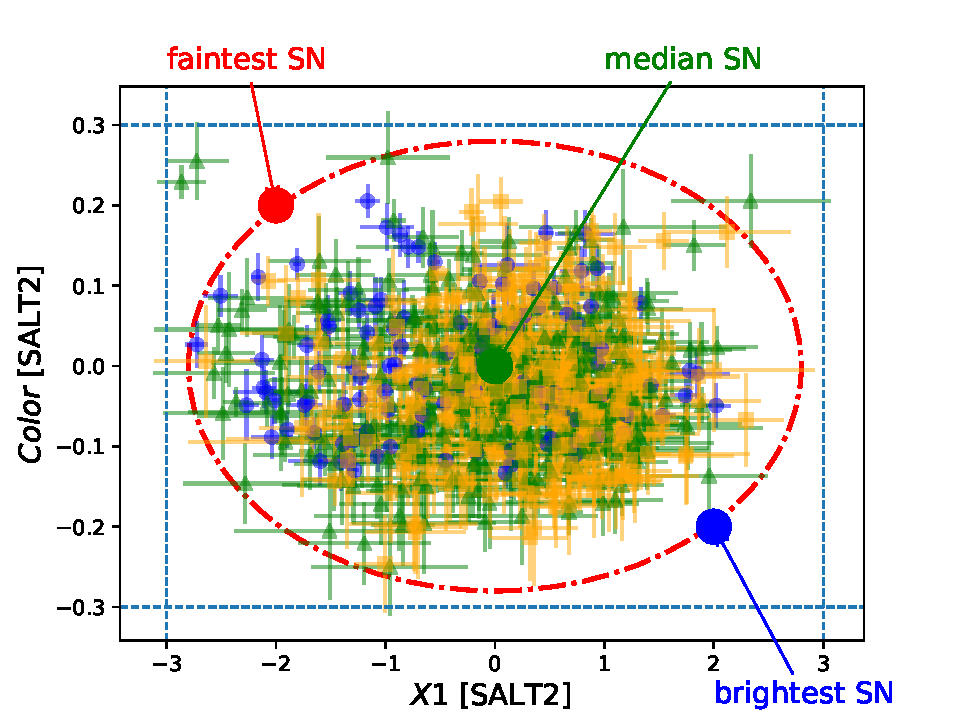
\includegraphics[width=0.6\textwidth]{Figures/sn_parameter_space.pdf}
    \caption{JLA supernovae the $(X_1,Color)$ parameter space --
      (blue: nearby, green: SDSS, orange: SNLS).  The large dots
      indicate the position of the faint, median and bright fiducial
      SNe used for the cadence analyses.}
    \label{fig:jla_X1_C}
  \end{center}
\end{figure}

On the same figure, we have represented three fiducial SNe of
particular interest: the red dot represents the faintest SN in this
region of the parameter space $(X_1=-2, C=0.2)$, the green dot and
blue dots show the average $(X_1=0, C=0)$ and brightest SN $(X_1=2,
C=-0.2)$ respectively.

We can define the redshift limit \zfaint as the limit beyond which the
faintest fiducal SN no longer passes the light curve requirements. By
doing this, we ensure that all SNe that live in the fiducial $(X_1,C)$
parameter space and are below \zfaint do pass our light curve
requirements.  \zfaint defines a {\em redshift-limited sample} whose
selection function does not depend on the SN properties.

We can also define a similar limit, using the median supernova,
instead of the faint one.  This defines a SN sample whose upper
redshift bins are affected by a selection bias, which must be
determined using a simulation -- which itself depends on our knowledge
of the SN luminosity distribution at those redshifts.  The uncertainty
affecting the determination of the selection function generally limits
the usefulness of the redshift bins affected by a selection bias.
Since the selection function is generally symmetric around its 50\%
point, the size of the sample limited by \zmed gives a good
approximation of the total number of LSST SNe that will have precise
distances.


\subsection{Metrics}

We propose to use as our primary metrics the size and depth of the
subset of well sampled SNe.  More precisely, we estimate, for each
cadence, the following quantities:

\begin{itemize}
\item the sample redshift limit, \zfaint defined above, and the number
  of well sampled supernovae below the redshift limit \nsnfaint
\item the redshift \zmed at which the median supernova defined above
  no longer passes the signal-to-noise requirements, and the number of
  well-sampled supernovae below this redshift, \nsnmed.  
\end{itemize}
The former give an assessment of the size and depth of the redshift
limited sample, i.e. the sample of supernovae usable for cosmology,
and whose selection function is extremely easy to determine.  The
latter gives an assessment of the size and depth of the sample of SNe
that will have precise distances.


\section{Method}

\subsection{Deep Drilling fields}
The DDF  observations involve a  small number of fields  and $O(10^4)$
SNe. The list of DDF simulated is given in table
\ref{tab:ddf_list} and on figure \ref{fig:ddf_map}. The location of four DDF (referred to as reference fields in the following: \cosmos, \xmmlss, \cdfs and \elais) has already been chosen by the project. The number of considered DDF ranges from 4 to 9.


\begin{table*}[!htbp]
  \begin{center}
  \begin{tabular}{|l|c|c|c|c|}
    \hline
    Field name & OpSim ID & Ra (deg) & Dec(deg) & Observing strategies\\
    \hline
    \cosmos & 2786 & 150.36 & 2.84 &All \\
    \xmmlss & 2412 & 34.39 & -5.09 & All \\
    \cdfs & 1427 & 53.00 & -27.44 & All \\
    \elais & 744 & 0.  & -45.52 & All \\
    \spt & 290 & 349.39 & -63.32 & All except feature*\\
    \ddfa & 820 & 119.55 & -43.37 & kraken\_2035\\
    \ddfb & 858 & 187.62 & -42.49 & kraken\_2035\\
    \ddfc & 1200 & 176.63 & -33.15 & kraken\_2035\\
    \ddfd & 2689 & 201.85 & 0.93 & kraken\_2035\\
    \hline
  \end{tabular}
  \caption{List and location of Deep Drilling Fields observed.}\label{tab:ddf_list}
  \end{center}
\end{table*}


\begin{figure}[htbp]
\begin{center}
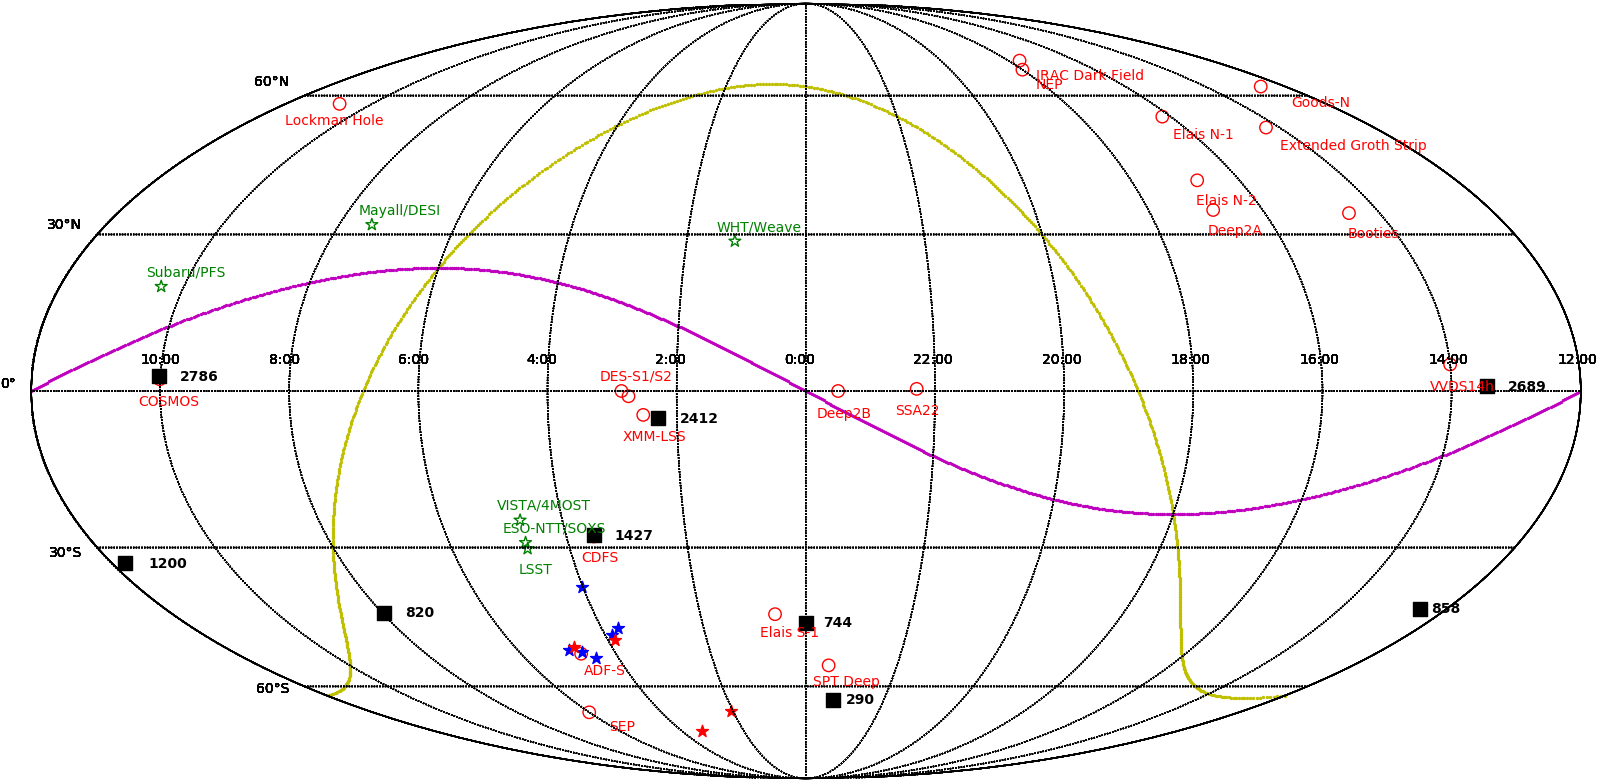
\includegraphics[width=14cm,height=10cm]{Figures/All.png}
\caption{Location of the Deep Drilling fields observed (black squares). Deep fields observed by previous surveys (red circles) and potential candidates for spectroscopic follow-up (green stars) are also mentioned. Yellow and magenta lines represent the Galactic and Ecliptic planes, respectivelly. Blue and red stars indicate potential deep field locations for EUCLID and WFIRST, respecivelly.}\label{fig:ddf_map}
\end{center}
\end{figure}

DDF observations are composed of sequences of 96 visits (in a row) in r,g,i,z,y bands (namely 20,10,20,26,20 visits). This corresponds to a total observing time of about one hour and few minutes if filter changes, slew times and telescope overheads are taken into account.

The strategy to estimate the number of well-measured type Ia supernovae may be summarized in four steps: (1) light curves are simulated and fitted using observations of a given cadence; (2) selection criteria are applied to get high-quality supernovae; (3) the resulting observing efficiency curves are then convolved with a production rate \cite{perrett} so as to estimate the number of well-measured type Ia supernovae that may be collected by LSST given an observing strategy. 

Table \ref{tab:sim_ddf} summarizes the parameter used in SN simulations. The selection of a sample of well-measured type Ia supernovae is done in two steps. A sample of observable supernovae is selected by requiring light curves to have \phasemin $\leq$ -5 and \phasemax $\geq$ 20 (where \phasemin~ and \phasemax~ are the minimal and maximum phases of the LC points, respectivelly). For each supernovae in this reference sample, additional selection criteria are applied:
\begin{itemize}
\item $N_{bef} \geq 4$ and $N_{aft} \geq 10$ where $N_{bef}$ and $N_{aft}$ are the number of LC points (with SNR$\geq$ 5) before and after \daymax.
 \item $\sigma_c \leq 0.04$ where $\sigma_c$ is the error on the \sncolor~parameter estimated from the fit of the light curve.
\end{itemize}
The season length which depends on the redshift is estimated using the supernovae of the reference sample.

\begin{table}[!htbp]
\begin{center}
\begin{tabular}{|c|c|}
\hline
Parameter & Range \\
\hline
                    & (-2.0,0.2),(0.0,0.0),(2.0,-0.2) \\
 (\strech,\sncolor) & (-2.0,0.0),(-2.0,0.2),(0.0,-0.2) \\
                    & (0.0,0.2),(2.0,0.0),(2.0,0.2) \\
\hline
\redshift           & [0.01,1.3] (step: 0.025) \\
\hline
\daymax             & [\tmin,\tmax] (step: 1 day) \\
                    & (\tmin~and \tmax~ are the min and max MJD of a season) \\
                    \hline
\end{tabular}
\caption{Range of the parameters used to simulate type Ia SN}\label{tab:sim_ddf}
\end{center}
\end{table}


\subsection{Wide Fast Deep}
WFD observations involve a large number of fields.  The observations
are dithered, and the size and depth of the final sample depends
heavily on the details of the observing strategy (in particular, the
filter allocation strategy and the field selection function \ldots)
For this reason, we opted for a slightly different approach, which we
describe below.

The celestial sphere is pixellized in Healpix superpixels\footnote{we
  choose nside=64, which corresponds to 0.8 deg$^2$ healpixels.  We
  have verified that (1) larger pixels (nside=32) leads to
  underestimating the number of SNe by ~ 15\% \FixMe{recheck that} and
  that smaller pixels (nside=128 and above) give exactly the same
  results.}.  Using a simple model of the LSST focal plane, we play
the cadence, and determine, the list of superpixels observed for a
given exposure. This allows us to build a log which reports the mjd,
band, and observing conditions of each healpixel observation.

We can then analyze this log, using as a probe, a fiducial SN~Ia,
e.g. the ``faint'' or ``normal'' SNe~Ia defined in the previous
section. For each mjd and each pixel, we determine:
\begin{eqnarray}
  z_{\mathrm{lim}} & = & \mathrm{max}\left(z | \mathrm{LC(z)\ fulfill\ requirements}\right) \\
  N_{z<z_{\mathrm{lim}}} &= & \delta\Omega_{\mathrm{pix}} \int_0^{z_\mathrm{lim}} \frac{\Delta T_{\mathrm{step}}}{1+z}\ {\mathcal{R}}(z)\ dV(z)
\end{eqnarray}
where $\delta\Omega_{\mathrm{pix}}$ is the solid angle subtended by
one pixel, $\Delta T_{\mathrm{step}}$ is the simulation time step (in
observer frame days) and $\mathcal{R}(z)$ is the SN~Ia volumetric rate
(we adopt the rate published in (Perrett et al, 2012)).  We also
compute the average cadence (in day$^{-1}$), i.e. the number of $g, r,
i$ or $z$ visits in a fiducial restframe interval.

The quantities above are determined for each pixel and each night
(identified by its mjd).  We report them in full sky maps, which give
an assessment of how the cadence performs in a $\sim 50$ day time
interval around the current mjd. From these maps, we can build global
maps giving, as a function of the position on the sky (1) the density
of supernovae (2) the median maximum redshift (3) the median cadence.
We can also collate these maps in videos, that are useful to evaluate
the observing strategy as a function of time.

\begin{sidewaysfigure}
    \begin{center}
      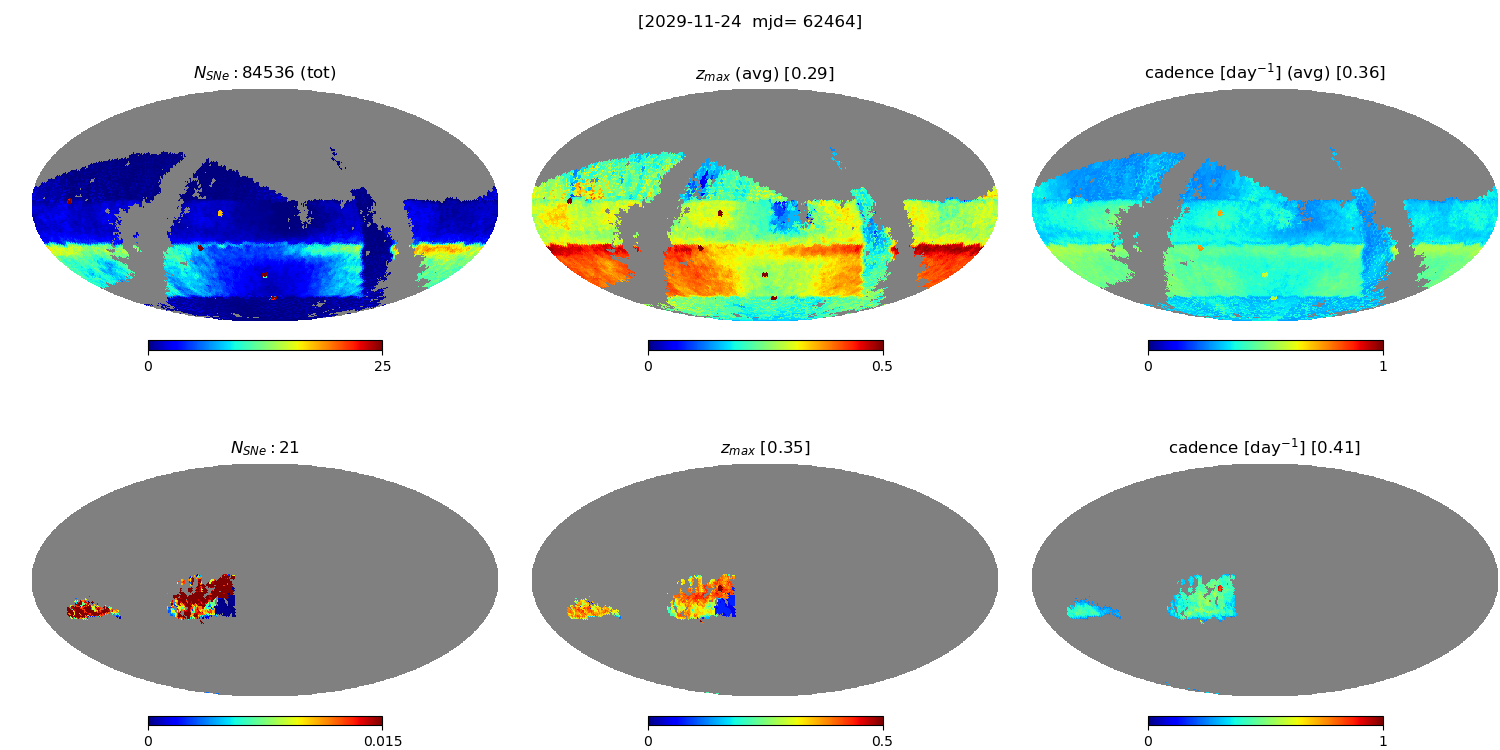
\includegraphics[width=\linewidth]{Figures/mothra_2045_02611.png}
      \caption{Example of cadence analysis maps.  Cadence {\em
          Mothra\_2045}, mjd=62464 (2029-11-24) {\em Upper panels:}
        (left) total number of well sampled supernovae per healpixel,
        (middle): median \zmed after 2611 days of survey, (right):
        median cadence, after 2611 days of survey. {\em Lower panels:}
        (left) number of SNe~Ia peaking at mjd=62464 and passing the
        light curve quality cuts (middle) \zmed, i.e.  maximum
        redshift at which a SN peaking at mjd=62464 would pass the
        requirements}
    \end{center}
\end{sidewaysfigure}


\section{Overview of observing strategies}

\subsection{Available strategies}

Four classes of observing strategies have been studied in detail:
\begin{itemize}

\item the {\tt OpSim}-based cadences released along with the white
  paper call (11 cadences released in June 2018 plus 4 additional
  simulations released in August), 
  
\item the {\tt OpSim}- and {\tt Feature}-based strategies that were
  available before the white paper call. 

\item simulations based on the {\tt Altsched} scheduler proposed by
  Stubbs and Rothchild.  This includes one rolling and another
  non-rolling cadence, plus a non-rolling simulation conducted on a
  larger footprint (P. Gris),

\item finally, we have tested a series of experimental observing
  strategies, based on the new feature-based scheduler (a.k.a.  SLAIR,
  Yoachim et al). These variations were produced by P. Yoachim, the
  main author of SLAIR, based on discussions we had at the summer 2018
  DESC week (CMU) and the 2018 LSST community workshop (Tucson).
\end{itemize}

In table \ref{tab:global_cadence_strats} we report, for each cadence
the total number of exposures per filter. This gives a general idea of
the total open shutter time, and the global filter allocation.  In
table \ref{tab:sn_specific_cadence_stats}, we show SN-specific key
statistics, in particular, the median number of visits in each filter,
for a given location of the sky (e.g. a healpixel), the median cadence
delivered by the observing strategy, the median season duration and
the total footprint of the survey.

As can be seen from tables \ref{tab:global_cadence_strats} and
\ref{tab:sn_specific_cadence_stats}, the proposed observing strategies
differ on a few key quantities:

\paragraph{Global filter allocation} All \opsim and \slair cadences   share the same global filter balance: 
$\sim 7\%, 10\%, 22\%, 22\%, 21\%$ and $18\%$ of the open shutter time
are allocated to the $u, g, r, i, z$- and $y$ bands respectively.
\altsched makes a different choice, based on the fact that the
low-throughput of the LSST camera in $y$, combined with the high sky
brightness in that band limit the impact of $y$-band observations.
About half of the $y$-band observing time is therefore reallocated to
$g$, $r$ and $i$ and $z$ bands, the resulting filter balance is
therefore: 9\%, 11\%, 28\%, 18\% 26\% and 9\% ($ugrizy$ respectively).

\paragraph{Filter allocation strategy} Another key point, is how the filters are
changed during the night.  In this regard, very different strategies
have been implemented by the various schedulers proposed so far.  This
is illustrated on figure \ref{fig:hourglass_plot_filter_alloc}, which
shows the filter usage for strategies {\em Pontus 2002} and {\em
  AltSched rolling}.  {\em Pontus 2002} attempts to minimize the
filter changes during a night and in fact keeps observing in the same
filter over several nights.  Conversely, the \altsched family of
cadences attempt to switch for a different filter after each observing
block, so that each revisit of the same field is performed in a
different band.  This has a major impact on the effective cadence
delivered by the survey. As of today, most \opsim cadences released so
far try to minize the number of filter changes, all \altsched cadences
switch filters after each observing block, and \slair has been
experimenting with both strategies.

\begin{figure}
  \begin{center}
    \subfigure[Pontus 2002]{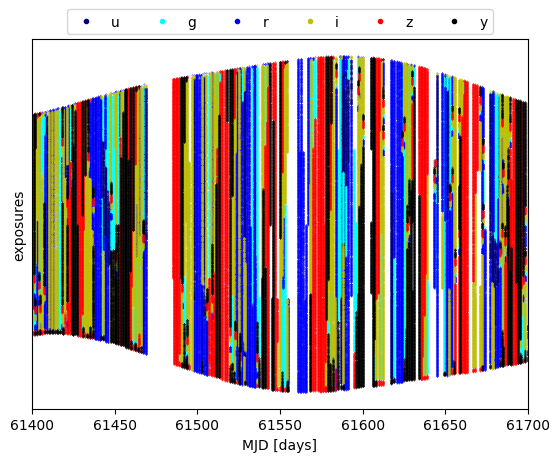
\includegraphics[width=0.48\linewidth]{Figures/pontus_2002_hourglass.png}}
    \subfigure[AltSched rolling]{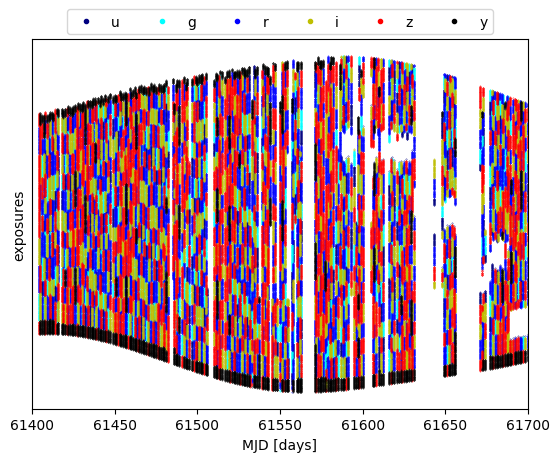
\includegraphics[width=0.48\linewidth]{Figures/alt_sched_rolling_hourglass.png}}
    \caption{Hourglass plots showing the filter usage for two
      different observing strategies. Most \opsim and \slair observing
      strategies released so far tend to minimize the number of filter
      changes. The AltSched strategy makes sure that each field is
      observed twice a night in different filter. This results in a
      higher number of filter changes, but is highly beneficial for
      the SN follow-up. }
    \label{fig:hourglass_plot_filter_alloc}
  \end{center}
\end{figure}

\paragraph{Visit pairs} In all cadences proposed so far (except a few experiments)
all fields are observed twice a night, 1 to 2 hours apart, in order to
improve the detectability of short term transients and solar system
objects.  Depending on the filter allocation strategy, this may have a
strong impact on the sampling quality of the SN~Ia light curves.
Indeed, SN~Ia luminosities vary significantly over time scales of one
to two days, and same band observations taken during a same night can
be considered as one single visit. When dealing with a fixed total
number of visits per sky direction, re-observing a field in the same
band during a night degrades the SN light curve sampling by a factor
$\sim 2$.  As an illustration, we show on figure
\ref{fig:effective_number_of_visits} show the median number of
effective visits visits for all cadences. The cadences that are best
for SNe~Ia are: 

%% On figure \ref{fig:effective_cadence}, we display the map of
%% effective cadences for

\paragraph{Season duration}



\paragraph{Rolling versus non-rolling cadences} 

\paragraph{Survey footprint}

\subsection{Key properties}


As a conclusion:

\subsubsection {WFD}

%% \begin{table}
%%   \begin{center}
%%     \begin{tabular}{}
%%       \hline
%%       \hline
%%       cadence & $u$   & $g$ & $r$ & $i$ & $z$ & $y$ \\
%%       \hline
%%       Minion  & $N_v$ & 
%%     \end{tabular}
%%   \end{center}
%% \end{table}

nb visits. n visits/night. Median internight gap. average cadence in a
given time window. season duration.

1 plot that gives the average cadence vs. season duration. 

Here, we show that clearly altsched dominates. 



\subsubsection{DDF}


All proposed observing strategies but altsched-like have included DDF.
Plots illustrating the four key points mentioned above are given on Figures \ref{fig:cosmos_cad}-\ref{fig:spt deep_m5} for baseline18a, feature\_baseline\_10yrs, kralen\_2026 and kraken\_2035 observing strategies and for the five to nine above-mentioned DDF. Among these cadences feature\_baseline\_10yrs displays interesting features with respect to supernovae observations for the reference DDF:
\begin{itemize}
\item Cadence: a median cadence of three days is observed whereas other observing strategies present cadences that may reach up to 14 days. Inter-night gaps are also smaller for \cosmos~and \xmmlss: 10 to 15 days and 5 to 7 days for the first and second maxima respectivelly whereas  for baseline18a, kralen\_2026 and kraken\_2035 the first (second) maximum is at the level of 18 to 40 (13 to 20) days.  
\item Season length: feature\_baseline\_10yrs shows the highest season lengths with values around 150 days for \cosmos~and \xmmlss, and 180 days for \cdfs and \elais whereas other strategies lead to values of about 130, 140, 120, and 150 for \cosmos, \xmmlss, \cdfs, and \elais, respectivelly.
\item Depth: while median m5-values are compatible among the strategies (the decrease during season 2 for the four fields in  feature\_baseline\_10yrs is due to a known bug in the weather simulations) the coadded m5 depth per season shows clearly that feature\_baseline\_10yrs is a 0.7 (\cosmos), 0.4 (\xmmlss, \cdfs, \elais) magnitude deeper (r-band) survey compared to the others. This results is to be explained by better cadences and longer seasons.
 
\end{itemize}
Key properties of \spt, \ddfa, \ddfb, \ddfc~and \ddfb~fields are given on Figures \ref{fig:spt deep_cad} to\ref{fig:kraken_m5}.


\section{ Results: Number of well-measured type Ia supernovae}

\subsection {WFD}

\begin{sidewaysfigure}
  \begin{center}
    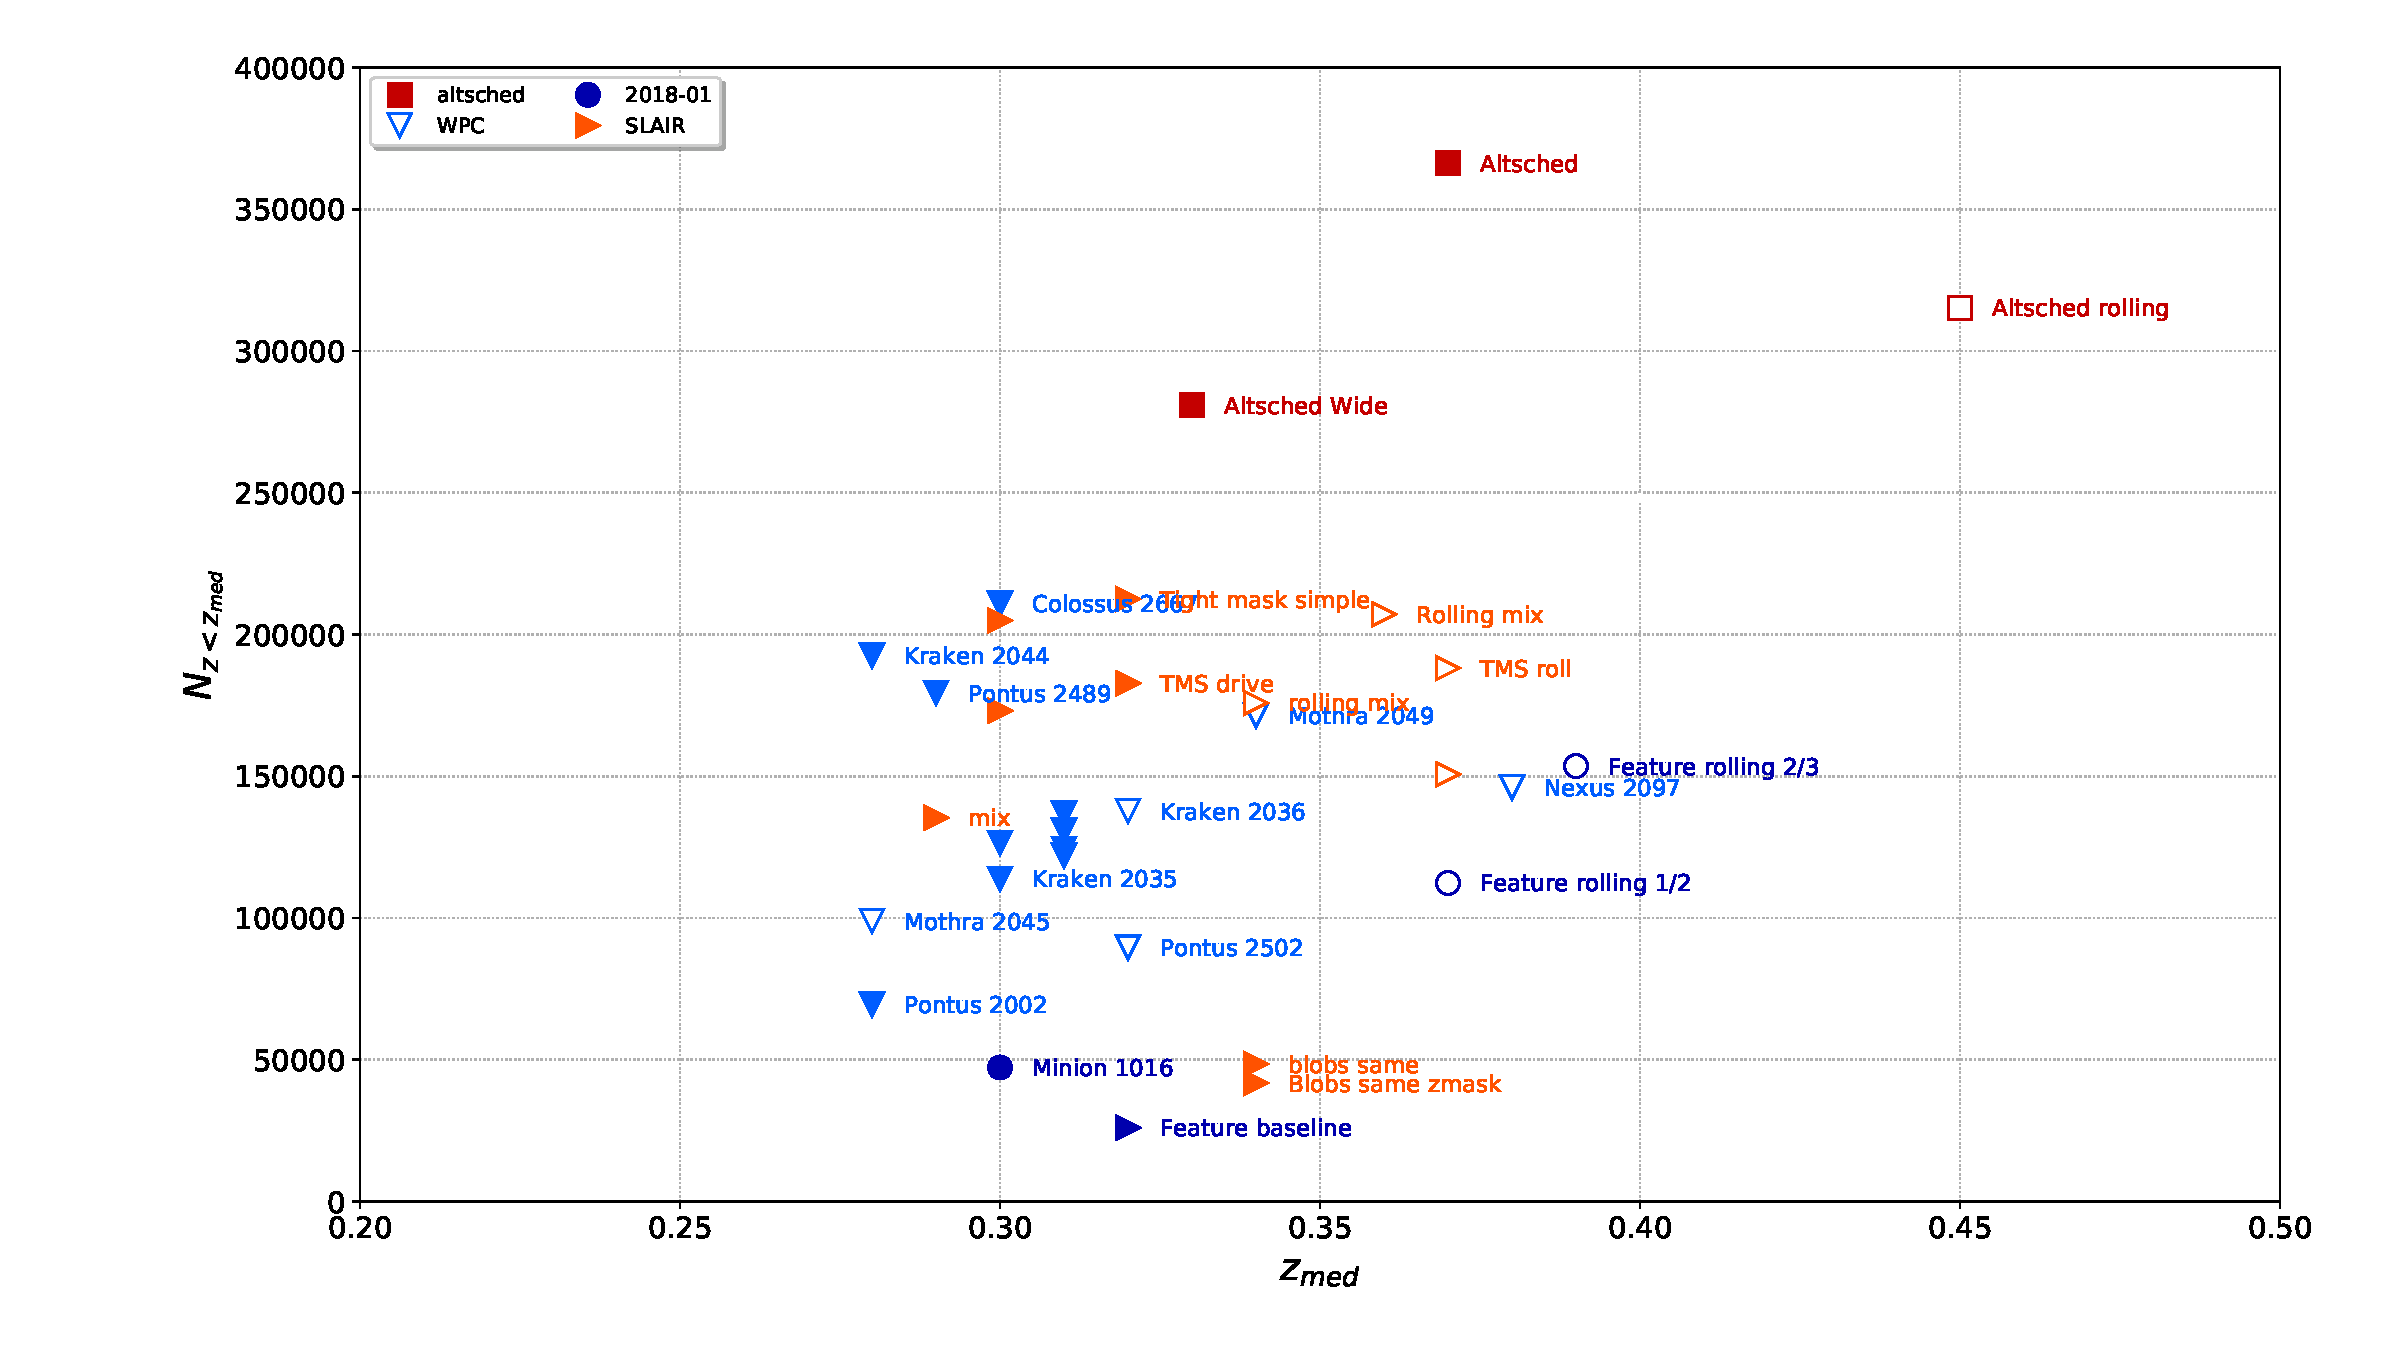
\includegraphics[width=\linewidth]{Figures/summary_plot_wfd_mediansn.pdf}
    \caption{Representation of the cadences analyzed in this study in
      the plane (\zmed, \nsnmed). This gives an assessement, for each
      cadence, of (1) the sample depth, i.e. at which redshift the
      median SN no longer passes the requirements listed in section
      \ref{sec:sn_sampling_requirements} and (2) the size of the
      subset of well-sampled SNe~Ia.}
  \end{center}
\end{sidewaysfigure}


\begin{sidewaysfigure}
  \begin{center}
    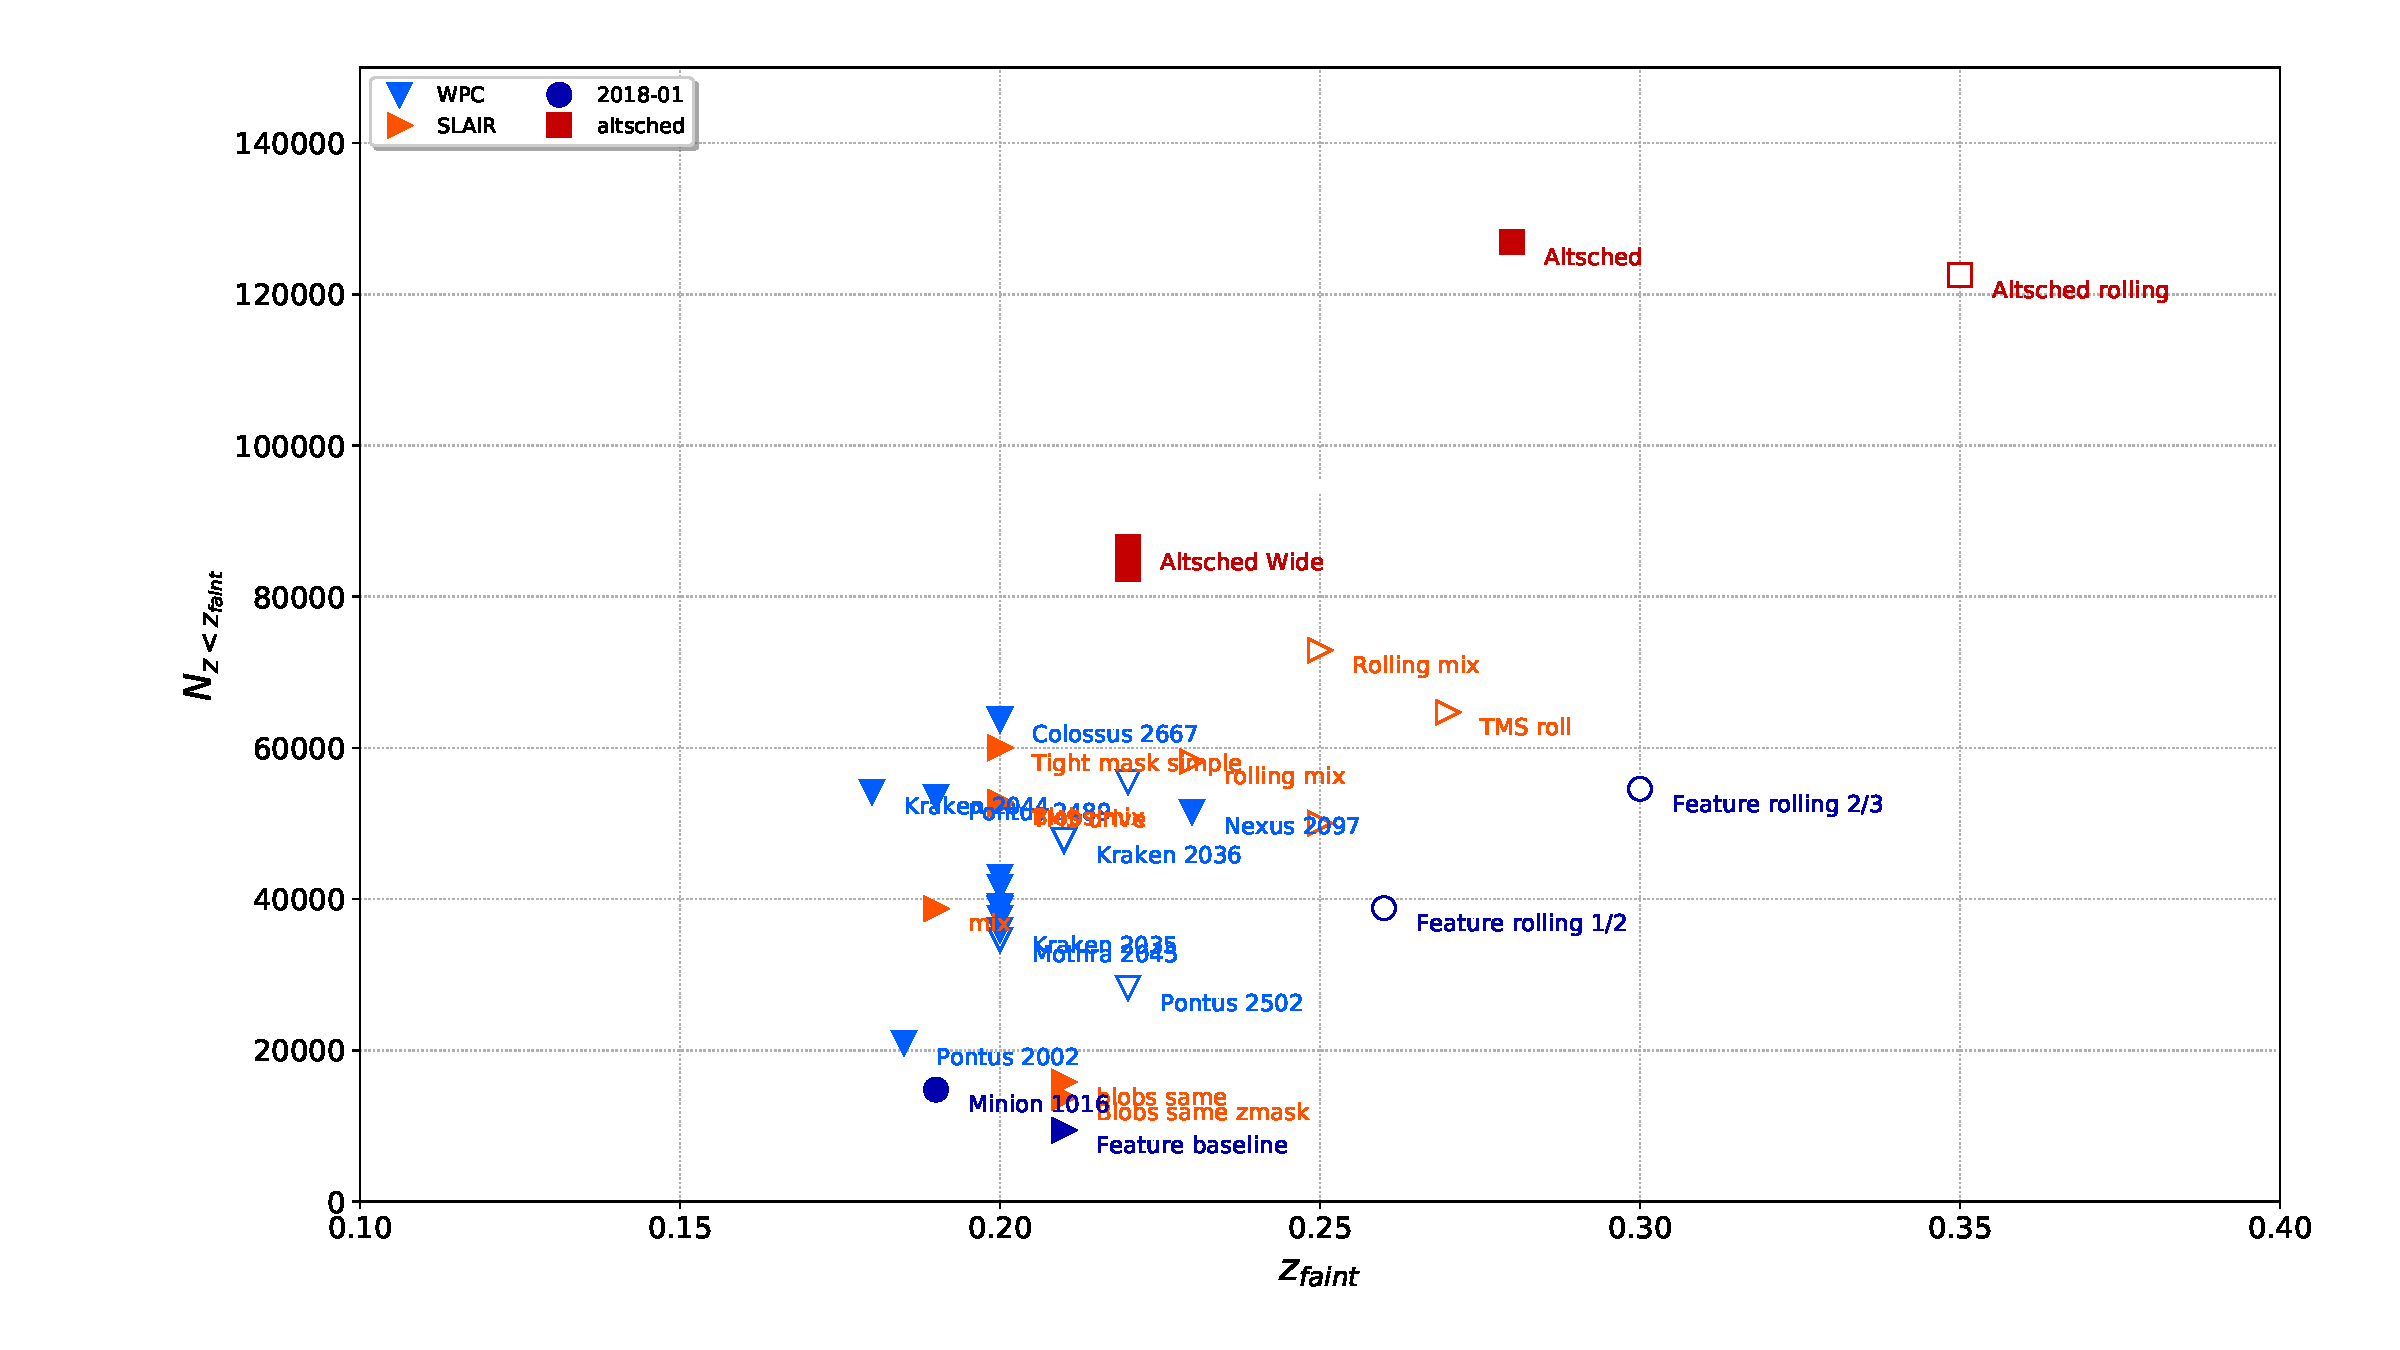
\includegraphics[width=\linewidth]{Figures/summary_plot_wfd_faintsn.pdf}
    \caption{Representation of the cadences analyzed in this study in
      the plane (\zfaint, \nsnfaint). This gives an assessement, for
      each cadence, of (1) the redshift limit of the survey, i.e. at
      which redshift the faintest SN no longer passes the requirements
      listed in section \ref{sec:sn_sampling_requirements} and (2) the
      size of the redshift limited SN~Ia sample produced by LSST.}
  \end{center}
\end{sidewaysfigure}

\subsection{ DD}

Typical detection efficiencies are given on Fig. \ref{fig:effi} for the \cosmos~field and feature\_baseline\_10 yrs cadence . One may observe that the lowest efficiencies (independently on the (\strech,\sncolor) values) correspond to the first two seasons of observations which are known to be very bad for this observing strategy and for this field (see for instance Figs. \ref{fig:cosmos_cad} and \ref{fig:cosmos_m5}).

\begin{figure}[htbp]
\begin{center}
  
  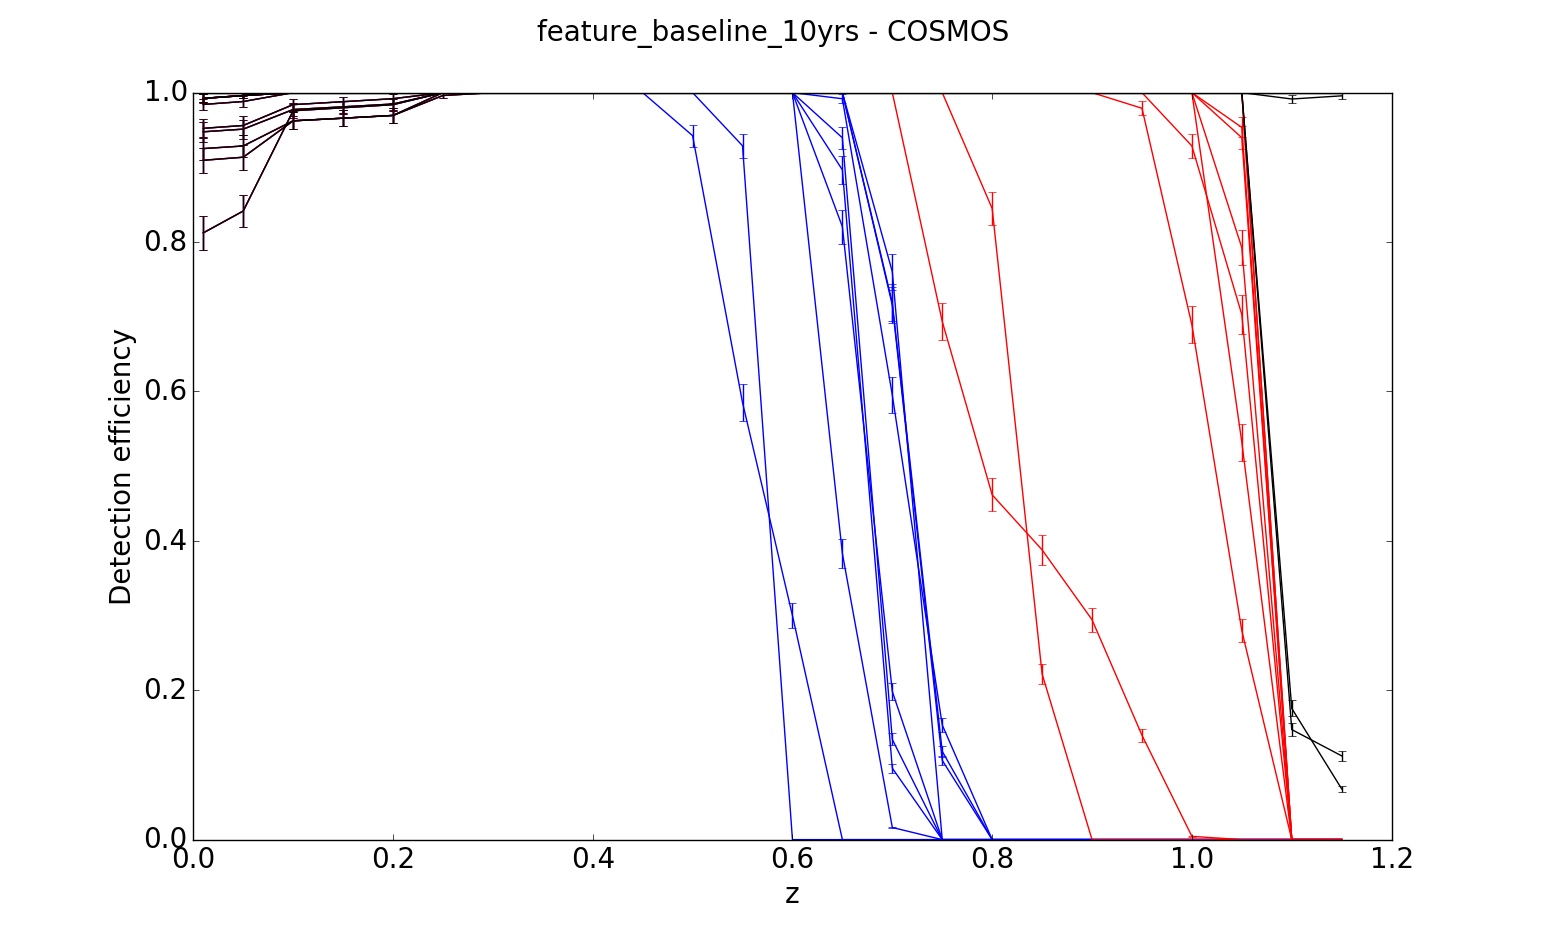
\includegraphics[width=12cm]{Figures/effi_feature_cosmos.png}
 \caption{Detection efficiency as a function of the redshift for the \cosmos~field and feature\_baseline\_10yrs observing strategy (10 seasons). Blue, red and black lines correspond to faint, medium and bright supernovae, respectivelly.}\label{fig:effi}
\end{center}
\end{figure}

Efficiency curves are convolved with a production rate \cite{perrett} to estimate the number of well-measured type Ia supernovae that may be collected by LSST. Summary plots are given for the reference fields (Fig \ref{fig:nsn_four}) and for all the DDF (Fig \ref{fig:nsn_all}). One may observe that, despite bad observing years, \feature~ shows the best results in terms of number of well-measured type Ia supernovae. Equivalent results are obtained with Colossus\_2667.

\begin{figure}[htbp]
\begin{center}
  
  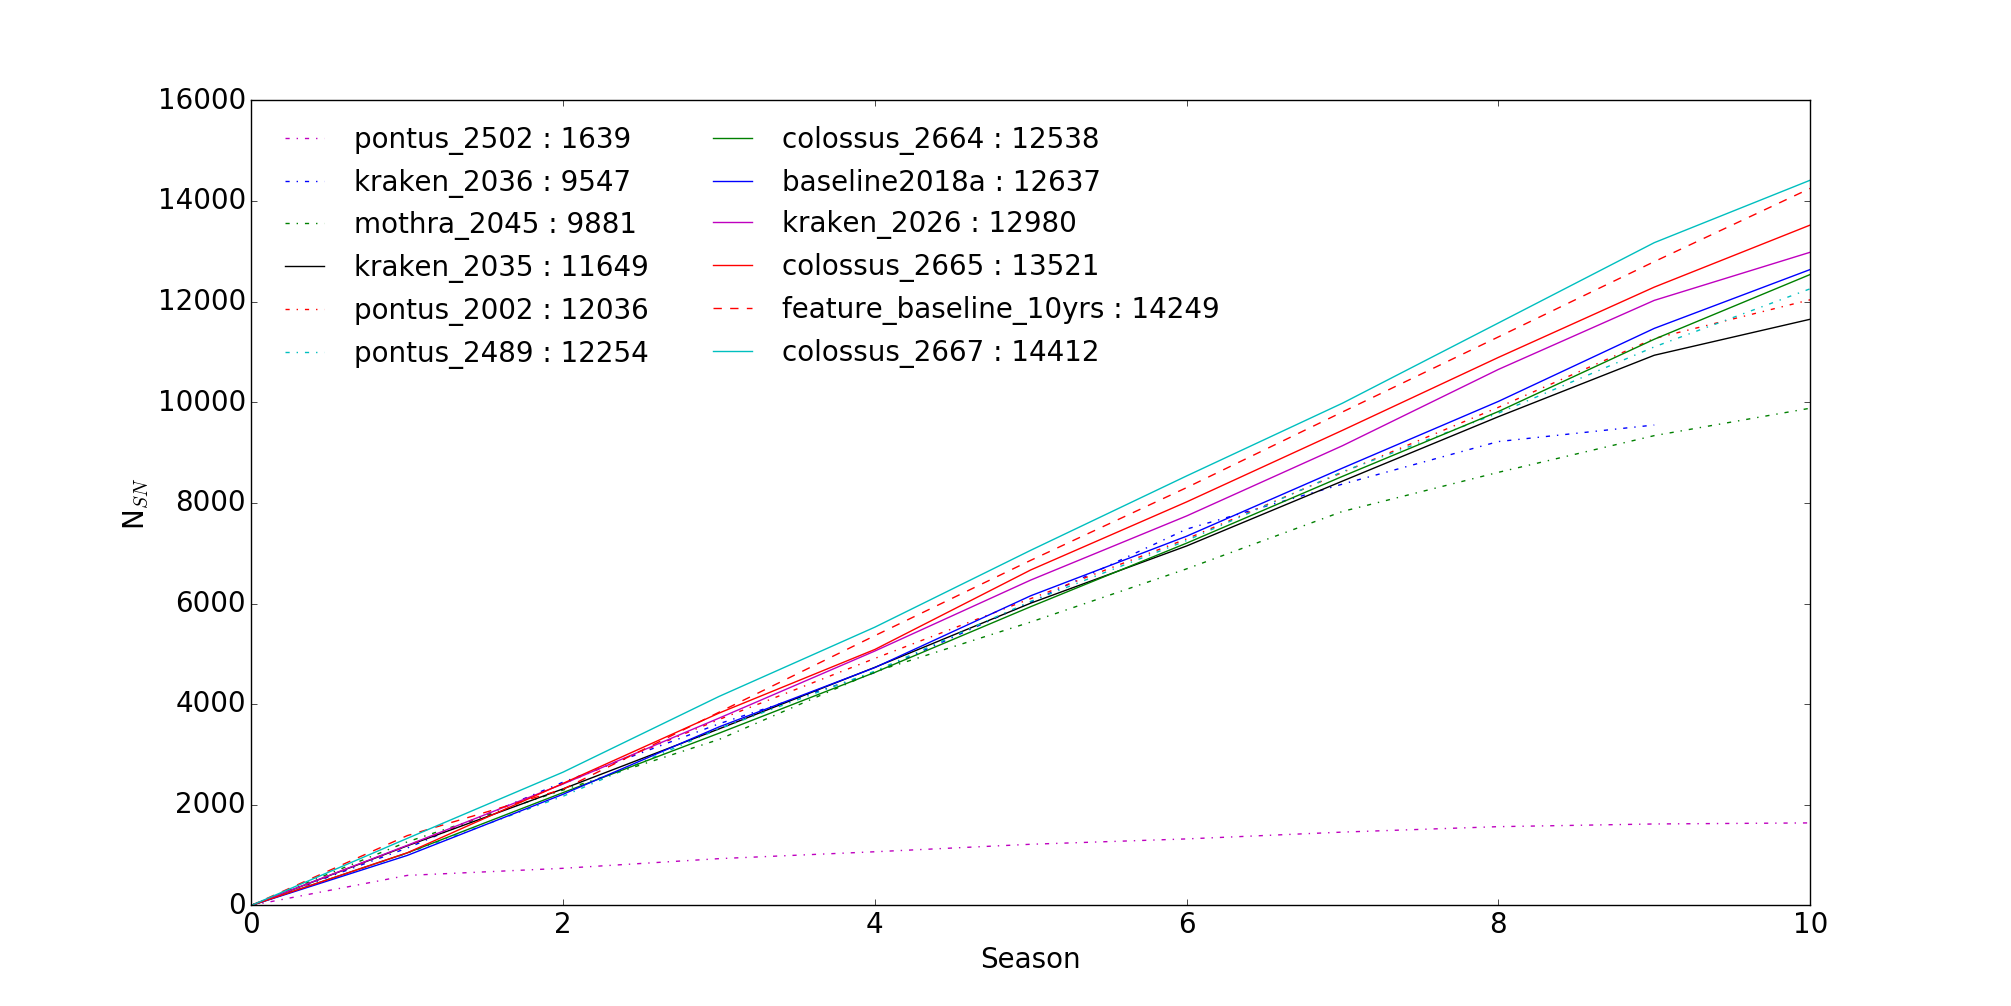
\includegraphics[width=15cm]{Figures/NSN_season_4DDF.png}
  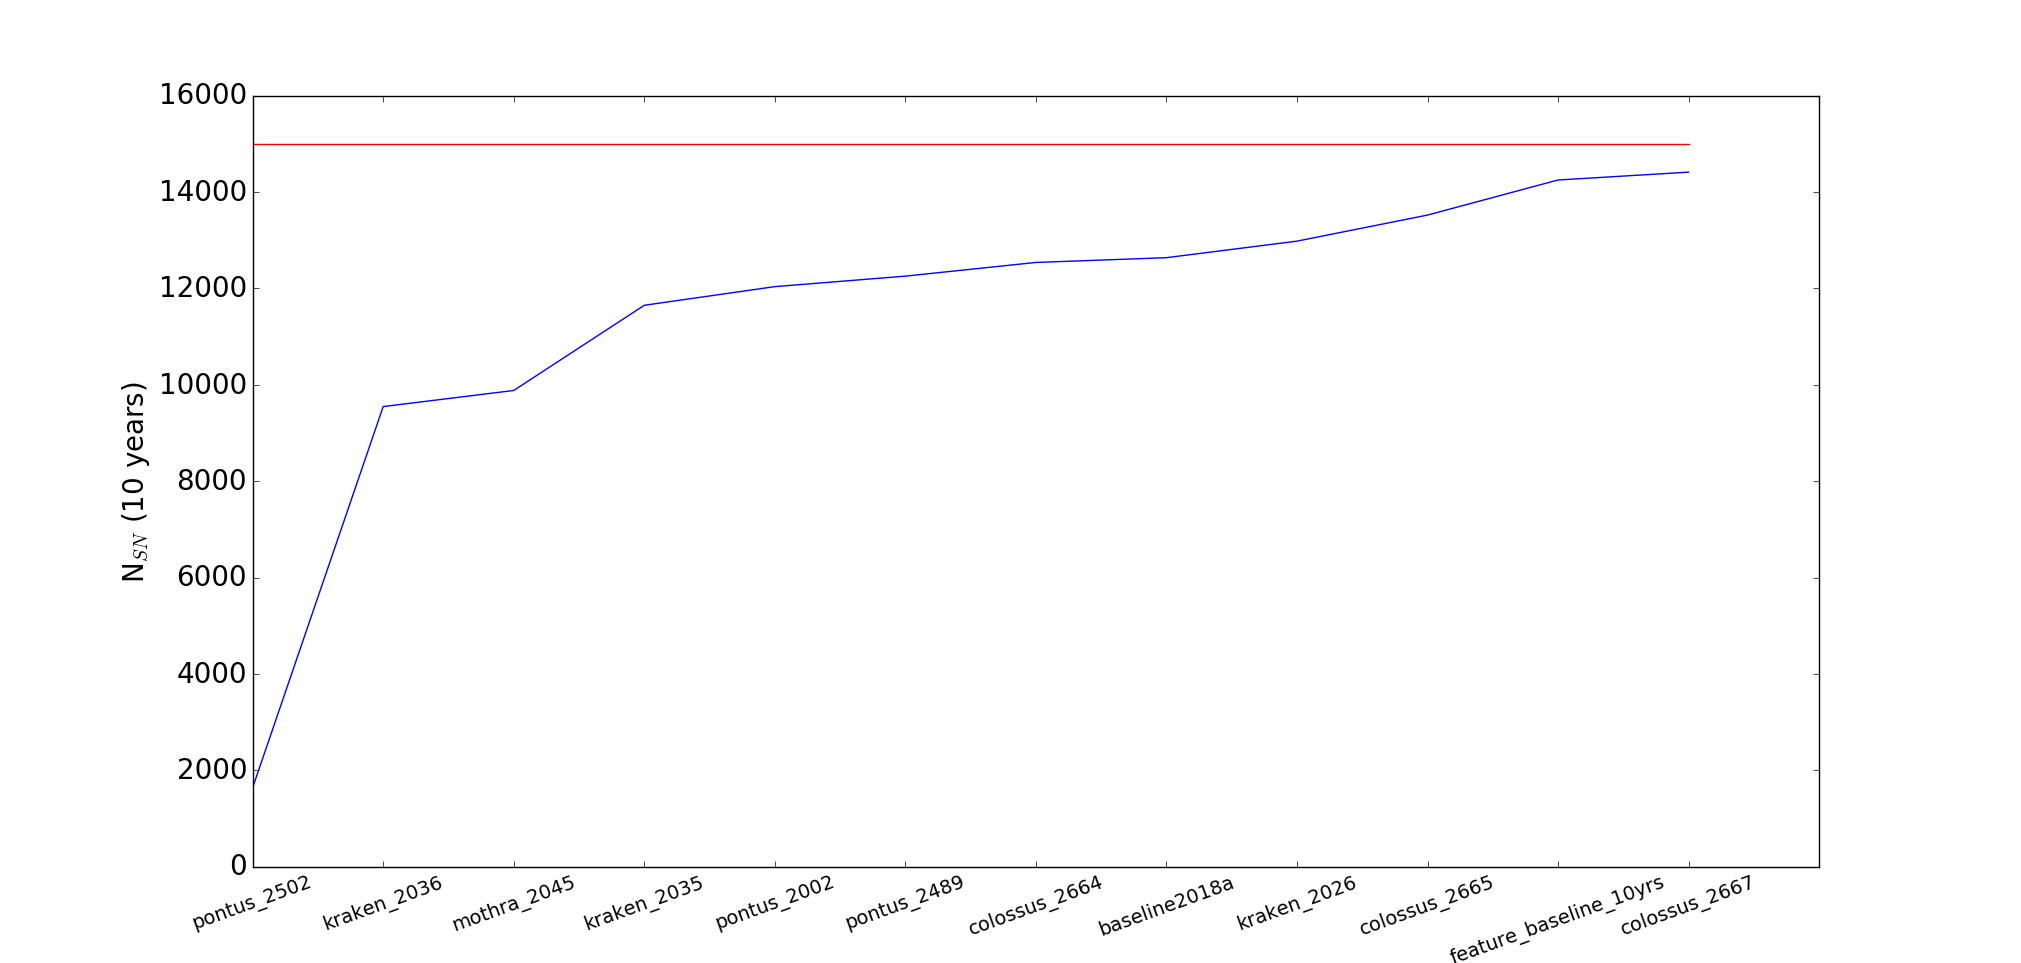
\includegraphics[width=15cm]{Figures/NSN_all_4DDF.png}
 \caption{Top: Number of well-measured type Ia supernovae as a function of the season. Bottom: Number of  well-measured type Ia supernovae as a function of observing strategy after ten years of operation. Four DDF (\cosmos,\xmmlss,\cdfs,\elais) have been considered. The red line corresponds to 15k supernovae.}\label{fig:nsn_four}
\end{center}
\end{figure}

\begin{figure}[htbp]
\begin{center}
  
  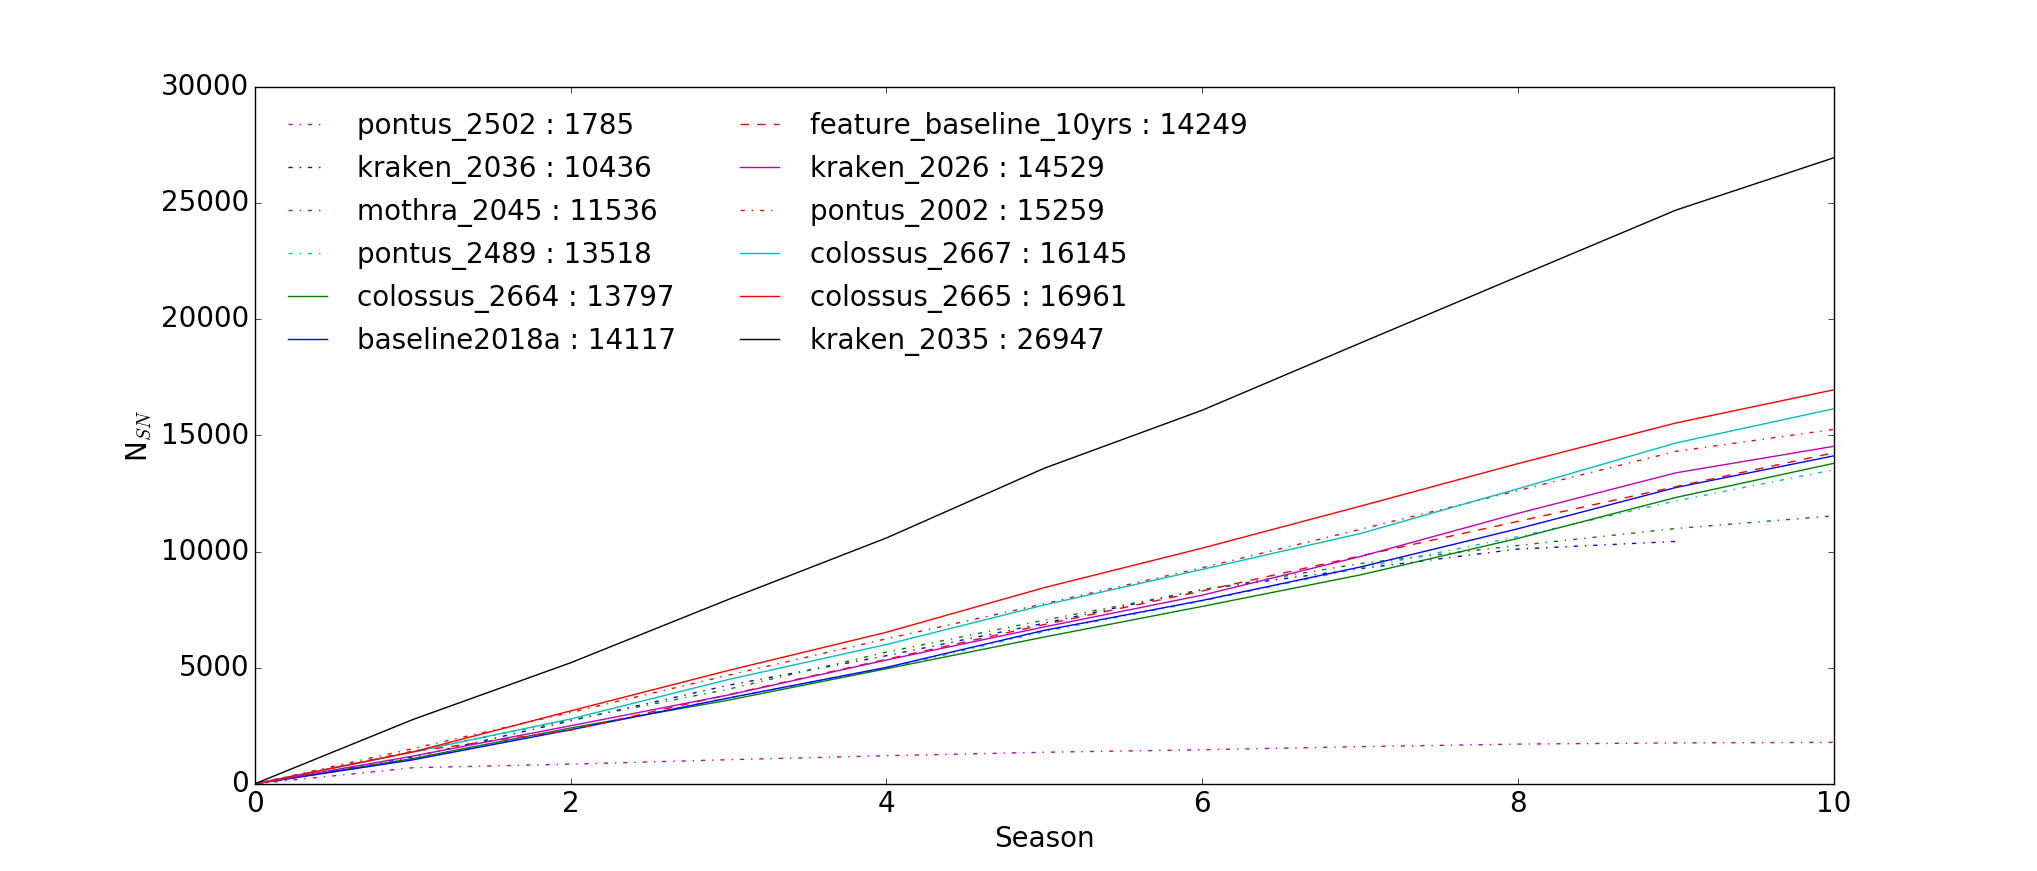
\includegraphics[width=15cm]{Figures/NSN_season_allDDF.png}
  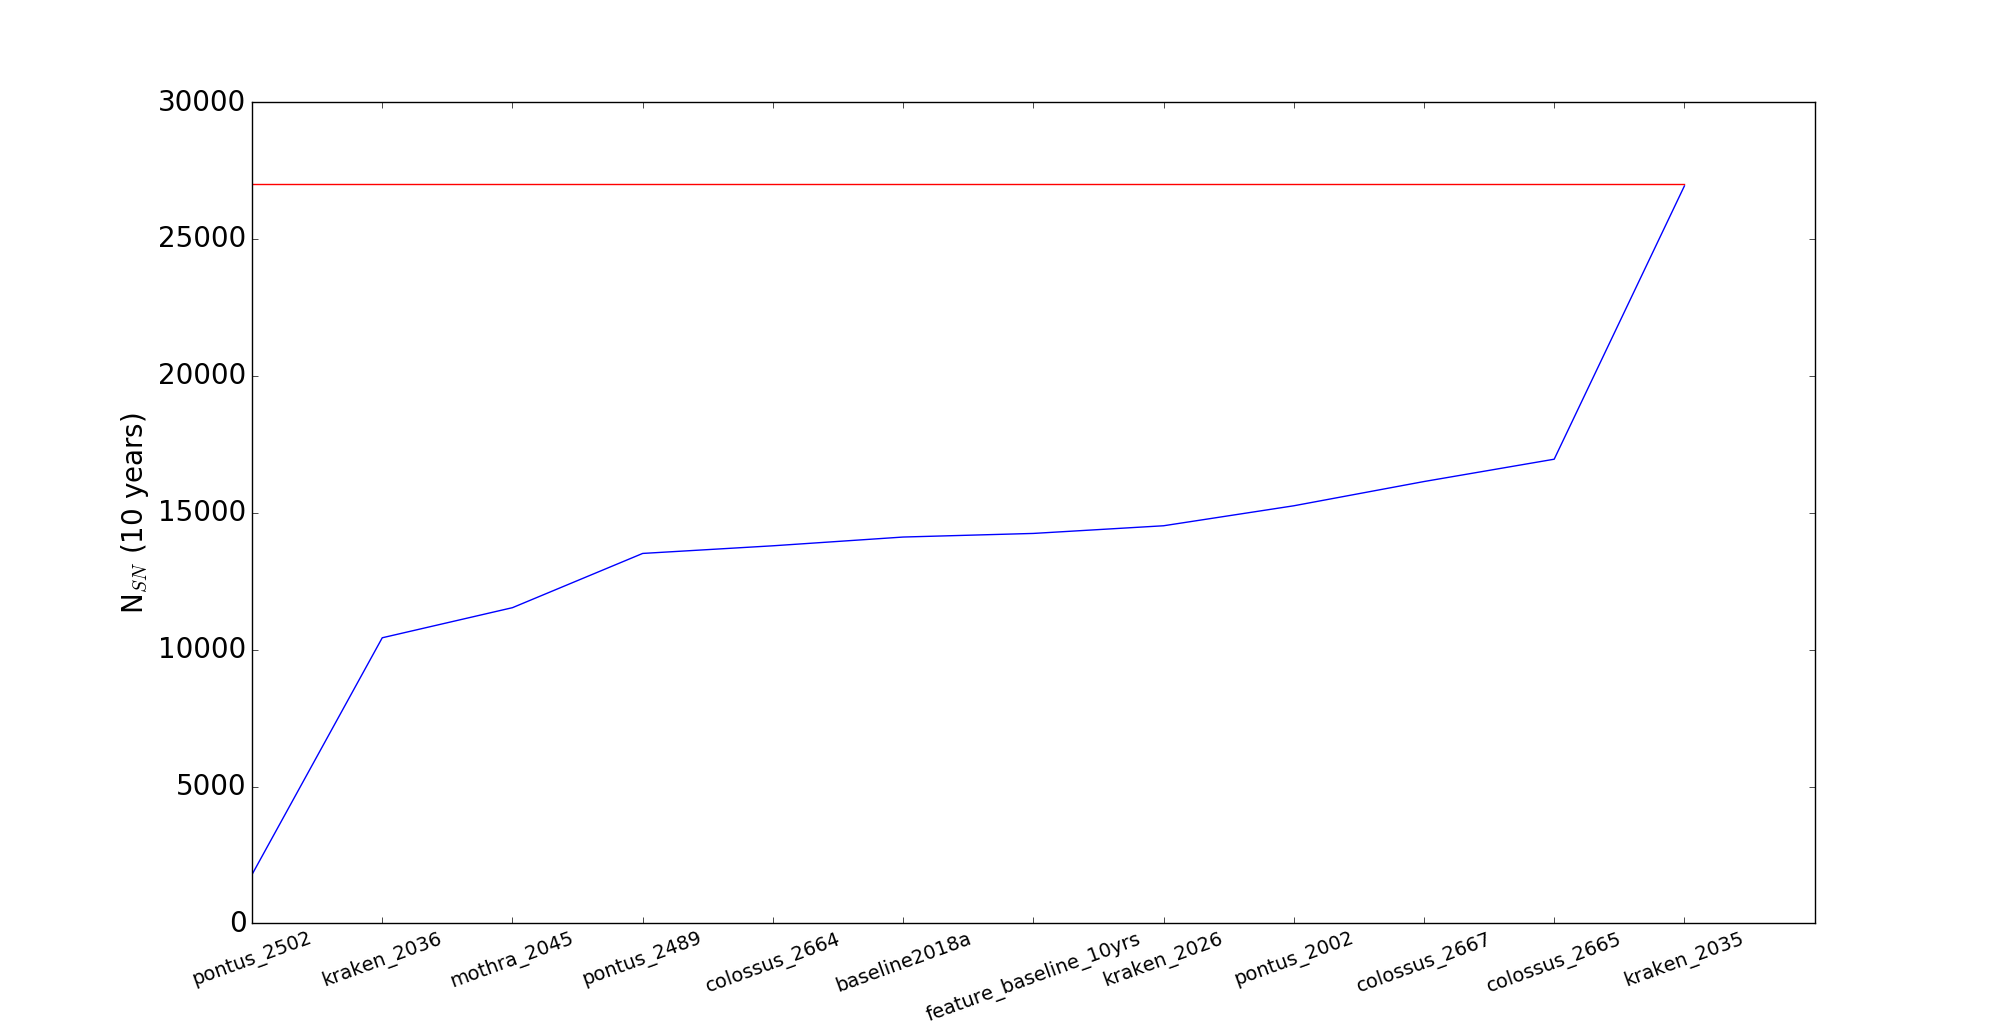
\includegraphics[width=15cm]{Figures/NSN_all_allDDF.png}
 \caption{Top: Number of well-measured type Ia supernovae as a function of the season. Bottom: Number of  well-measured type Ia supernovae as a function of observing strategy after ten years of operation. All DDF have been considered.The red line corresponds to 27k supernovae.}\label{fig:nsn_all}
\end{center}
\end{figure}

When considering all DDF the winner is of course kraken\_2035 (27K after ten years) since this observing strategy considered 9 DDFs whereas all others observed 4 to 5 fields. One may observe that extrapolating a four fields configuration results (like the ones obtained with \feature) to a 9 DDF observing strategy will probably lead to an overestimation of the resulting number of well-measured type Ia supernovae. It is indeed difficult to maintain the same quality (in terms of cadence, season length and thus depth) when moving from a 4 to a 9 DDF strategy.

\begin{figure}[htbp]
\begin{center}
  
  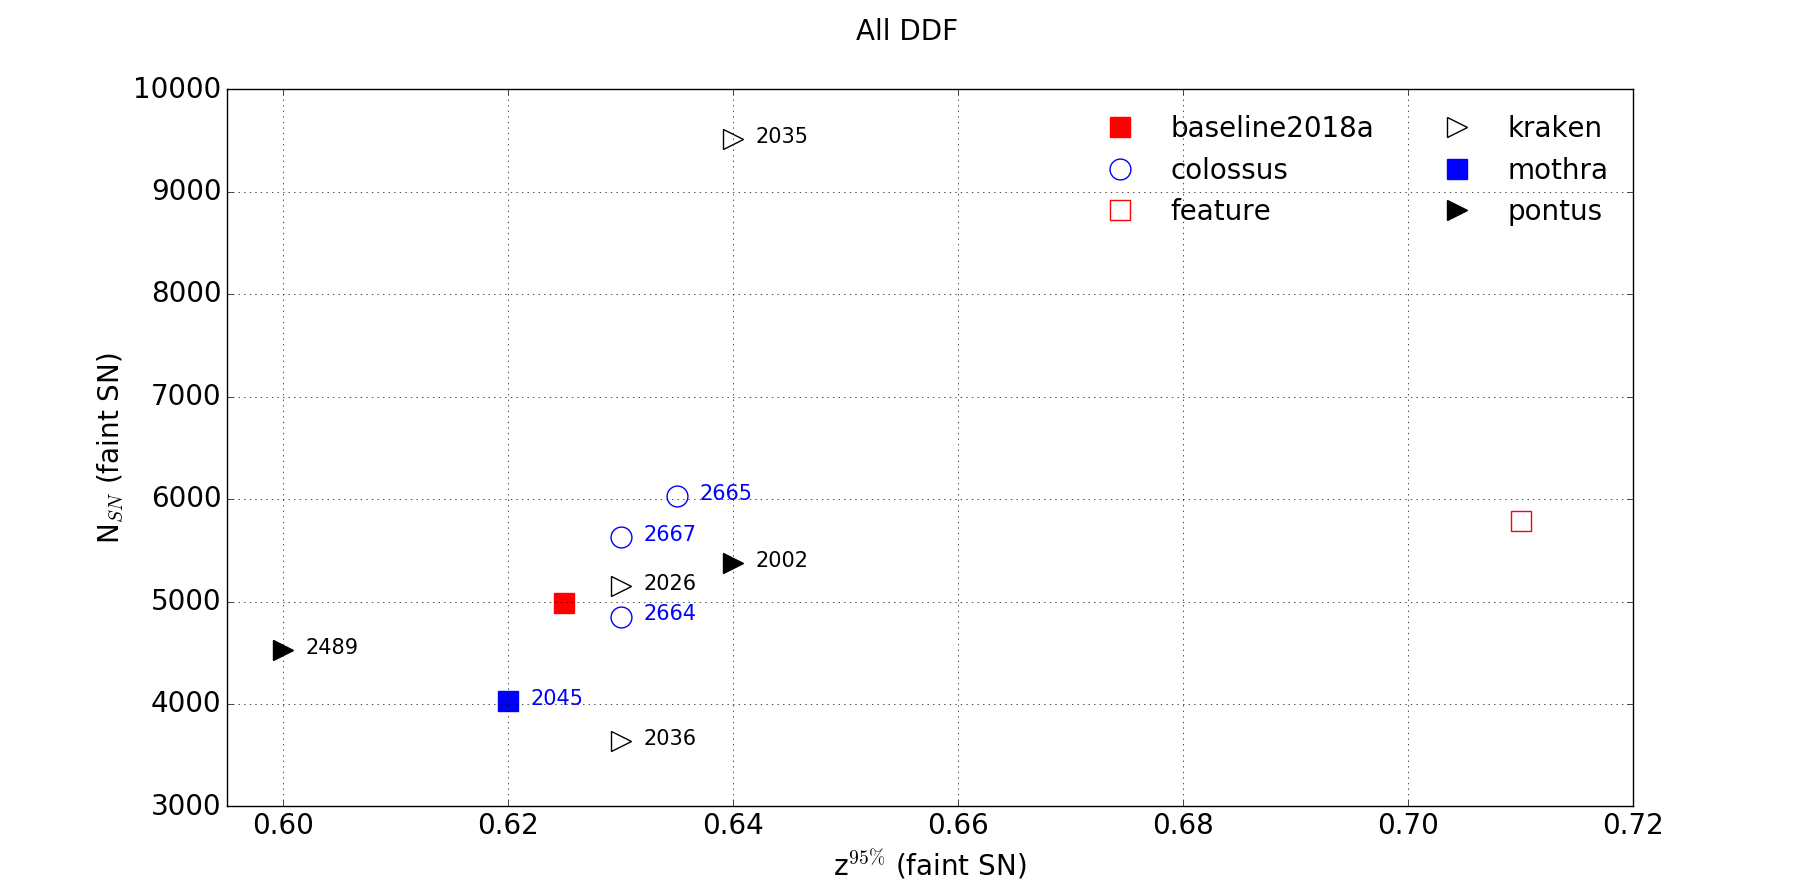
\includegraphics[width=15cm]{Figures/Z95_NSN.png}
 \caption{95\% redshift limit (ie corresponding to the detection of 95\% of the supernovae of the corresponding sample) as a function of the number of faint supernovae. Each point correspond to a field, a season and an observing strategy.}\label{fig:z95}
\end{center}
\end{figure}

Another way to assess the quality of an observing strategy is to estimate the redshift detection limit for faint supernovae (per season and per field). On Figure \ref{fig:z95} is displayed the 95\% redshift limit (ie corresponding to the detection of 95\% of the supernovae of the corresponding sample) as a function of the number of faint supernovae. Huge variations among and inside strategies are observed. This plot reflects the quality of the proposed cadences. It seems that \redshift~of 0.7-0.75 may be reached with four fields. Once again \feature~tend to give the highest redshifts and the most homogeneous results among the fields and seasons. 

\section{New proposals}

\subsection{DDF observing strategy}

In OpSim the choice to observe a given field is done on the fly according to an optimized selection function depending on criteria including (among others) observing conditions, slew time minimization, last time of visit, and total observing time. While the use of a simple metric (see below) would help in choosing another approach could be to use a pre-defined table that would specify which DDF are to be observed on a given night.

Let us consider the four reference fields \cosmos, \xmmlss, \cdfs~and \elais. Since the location are well known, it is possible to estimate when these fields are visible (that is with an altitude between 20 and 86.5 degrees) for a large enough period (typically 20 to 40 minutes) of good observing conditions (ie with airmass lower than a reference value - typically 1.5). We may define a (boolean) parameter dubbed observability equal to one when the above-mentioned conditions are filled, and 0 otherwise. This parameter is displayed on Figure \ref{fig:observability} (top). \xmmlss,\cdfs, and \elais~ are located in the same (Ra) region and may thus be observed during the same night whereas \cosmos~may be observed when all others are not visible. Season lengths of observability (Figure \ref{fig:observability} - bottom) range from 200 to 290 days.


\begin{figure}[!htbp]
\begin{center}
  
  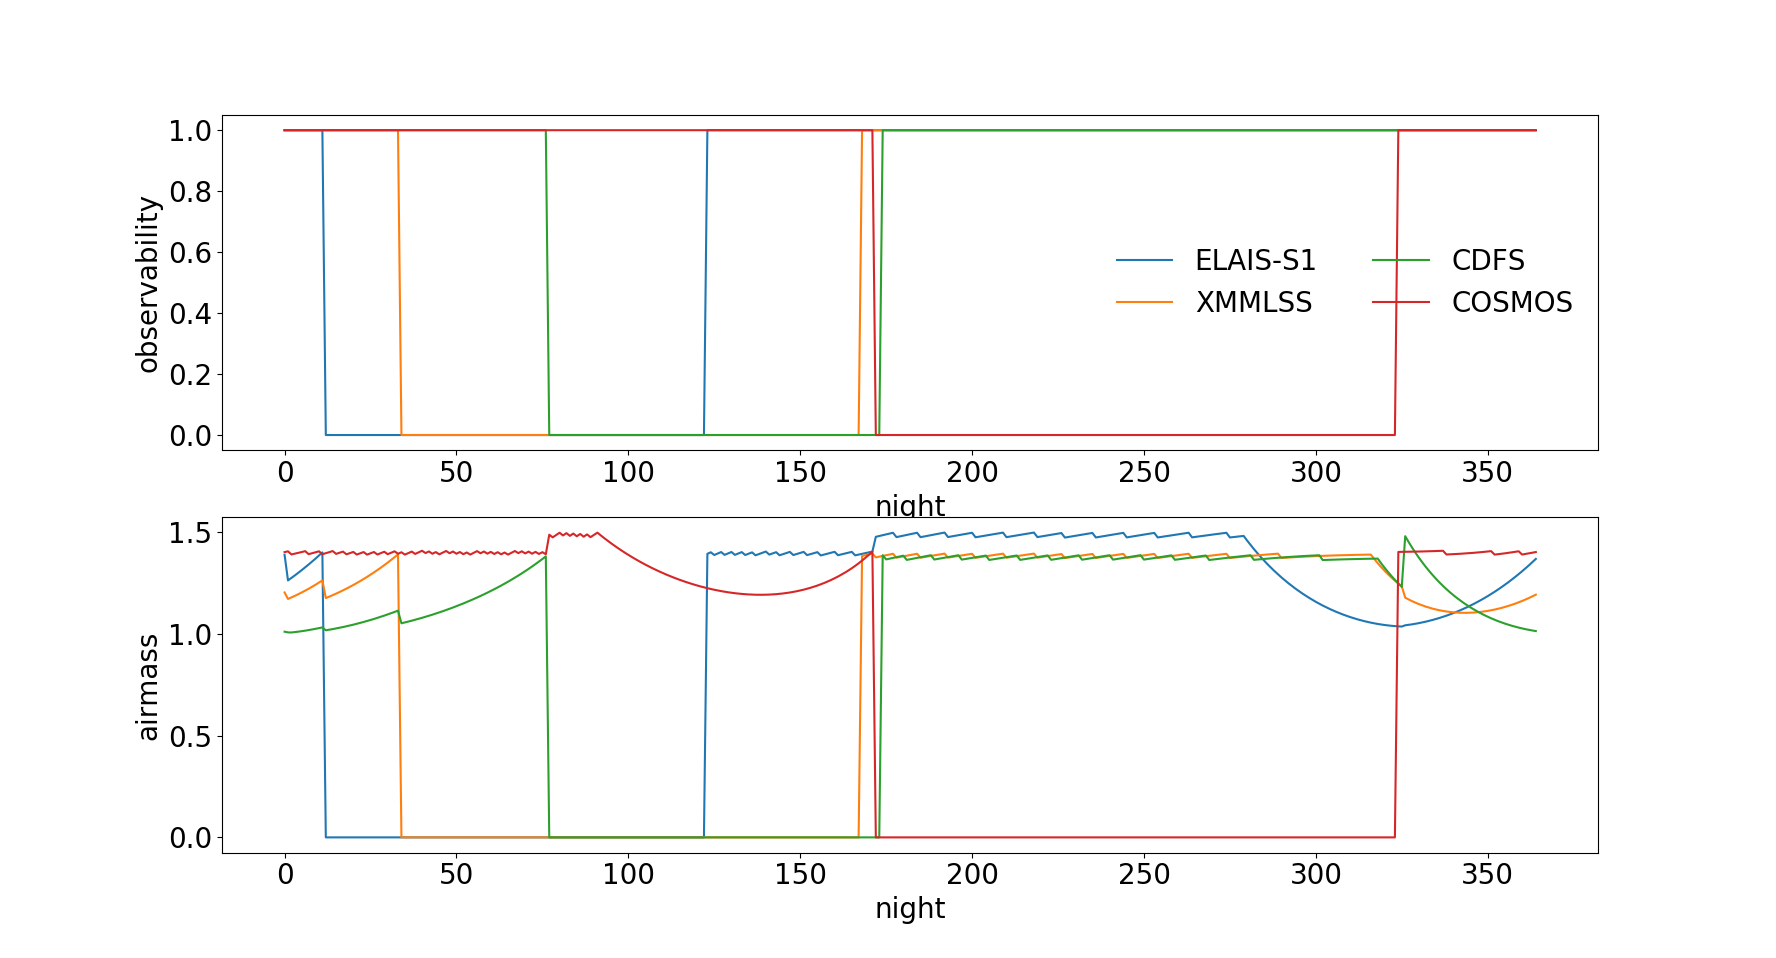
\includegraphics[width=18cm,height=12cm]{Figures/observability.png}
  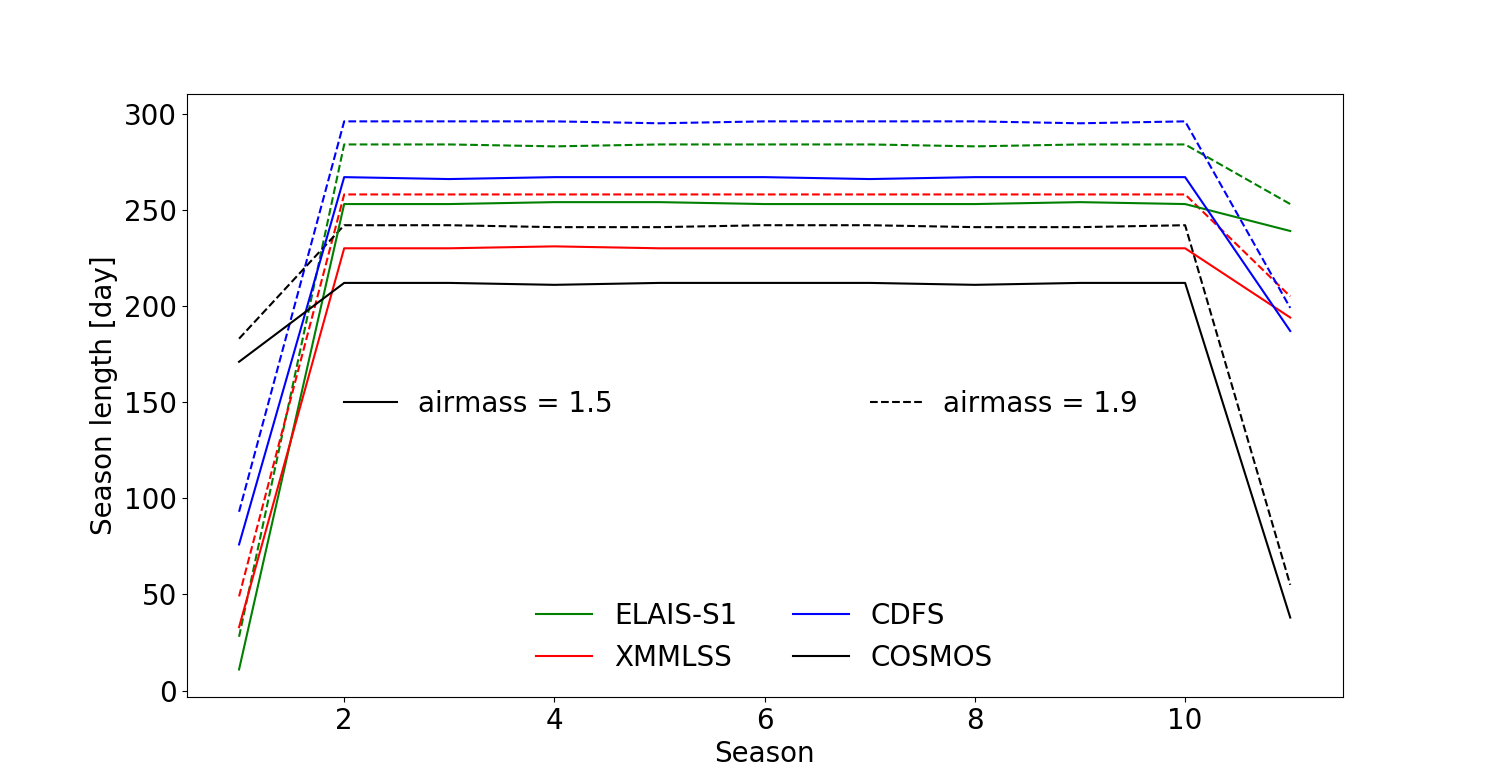
\includegraphics[width=18cm,height=8cm]{Figures/Season_length.png}
 \caption{Top: observability (see definition in the text) and airmass as a function of the night number (first year of LSST operation). Bottom: season length as a function of the season for an airmass limit of 1.5 (full lines) and 1.9 (dashed lines).}\label{fig:observability}
\end{center}
\end{figure}

The table of observations may be defined using median gap values \tgapcosmos~and \tgapothers~when \cosmos~and \xmmlss,\cdfs,\elais~are not observable, respectively. Observing time windows are then defined by:
\begin{itemize}
\item{[\tgapothers-w/2,\tgapothers+w/2]: \cosmos~ is observed}
\item{[\tgapcosmos-w,\tgapcosmos+w]: \xmmlss, \cdfs, \elais~are observed.}
\end{itemize}
with a width w equal to 2/3*(\tgapcosmos-\tgapothers).

\subsection{altsched rolling 80/20}

\subsection{altsched rolling 75/25}

\subsection{Adding a simple metric for SN in OpSim/SLAIR}

\section{ Conclusion}

\begin{thebibliography}{9}
\bibitem{perrett} Evolution in the Volumetric Type Ia Supernova Rate from the Supernova Legacy Survey, K.Perrett {\it et al}, The Astronomical Journal, Volume 144, Issue 2 (2012).
  
 \end{thebibliography}

\clearpage


\appendix
  


\begin{appendices}

\section{Derivation of formula \ref{eqn:snr}}

\label{sec:snr}

If we fit a light curve model $L(t) = A \times \ell(t)$ on a
lightcurve $(t_i, y_i, \sigma_i)$, the least square estimate of $A$ is
given by:
$$
\hat{A} = \frac{\sum w_i \ell_i y_i}{\sum w_i \ell_i^2}
$$
and the signal-to-noise ratio on $\hat{A}$ is:
$$
SNR = \sum_i (w_i L_i^2)^{1/2}
$$ since we are in the background dominated regime, the weights may be
expressed as a function of the $5-\sigma$ limiting flux of each visit
$f_{i|5}$, and we have:
$$
SNR_{\mathrm{band}} = \sum_{i} 5 \times (f^{-2}_{i|5} L_i^2)^{1/2}
$$
where $5-\sigma$ limiting flux of each visit $f_{i|5}$.


\section{Cadence global statistics}

%\begin{table}
%\begin{center}
  \begin{longtable}{l|ccccccc}
    \caption{Global filter allocation of all cadences studied in this note\label{tab:global_cadence_stats}}        \\
    
    \hline
    \hline    
  name & \multicolumn{7}{c}{\# visits} \\
       & $u$ & $g$ & $r$ & $i$ & $z$ & $y$ & Total \\

  \hline
  \hline
  \multicolumn{8}{c}{Cadences simulated for the White paper call}\\
  \hline      
      baseline 2018a &  177538 &  234144 &  515172 &  514481 &  486208 &  445157 &  2372700 \\ 
                     &    7.5 \% &    9.9 \% &   21.7 \% &   21.7 \% &   20.5 \% &   18.8 \% & \\
\hline
         kraken 2035 &  176828 &  237799 &  522679 &  520282 &  497539 &  454450 &  2409577 \\ 
                     &    7.3 \% &    9.9 \% &   21.7 \% &   21.6 \% &   20.6 \% &   18.9 \% & \\
\hline         
         kraken 2042 &  197391 &  258590 &  571414 &  567785 &  529266 &  484923 &  2609369 \\ 
                     &    7.6 \% &    9.9 \% &   21.9 \% &   21.8 \% &   20.3 \% &   18.6 \% & \\
\hline
         kraken 2036 &  150652 &  200360 &  441677 &  439015 &  443328 &  392881 &  2067913 \\ 
                     &    7.3 \% &    9.7 \% &   21.4 \% &   21.2 \% &   21.4 \% &   19.0 \% & \\
\hline
         kraken 2044 &  179340 &  230010 &  520373 &  519688 &  509678 &  492524 &  2451613 \\ 
                     &    7.3 \% &    9.4 \% &   21.2 \% &   21.2 \% &   20.8 \% &   20.1 \% & \\
\hline
         kraken 2026 &  182465 &  241422 &  532326 &  529190 &  496037 &  456948 &  2438388 \\ 
                     &    7.5 \% &    9.9 \% &   21.8 \% &   21.7 \% &   20.3 \% &   18.7 \% & \\
\hline
       colossus 2665 &  182959 &  238121 &  527822 &  524508 &  494317 &  458122 &  2425849 \\ 
                     &    7.5 \% &    9.8 \% &   21.8 \% &   21.6 \% &   20.4 \% &   18.9 \% & \\
\hline
       colossus 2667 &  185815 &  242738 &  534218 &  533143 &  517513 &  479169 &  2492596 \\ 
                     &    7.5 \% &    9.7 \% &   21.4 \% &   21.4 \% &   20.8 \% &   19.2 \% & \\
\hline
       colossus 2664 &  179185 &  237797 &  533279 &  530020 &  500969 &  459024 &  2440274 \\ 
                     &    7.3 \% &    9.7 \% &   21.9 \% &   21.7 \% &   20.5 \% &   18.8 \% & \\
\hline
         pontus 2502 &  128795 &  186756 &  421971 &  426707 &  370248 &  499345 &  2033822 \\ 
                     &    6.3 \% &    9.2 \% &   20.7 \% &   21.0 \% &   18.2 \% &   24.6 \% & \\
\hline
         pontus 2002 &  176036 &  228309 &  519417 &  518145 &  494484 &  489085 &  2425476 \\ 
                     &    7.3 \% &    9.4 \% &   21.4 \% &   21.4 \% &   20.4 \% &   20.2 \% & \\
\hline
         pontus 2489 &  242197 &  334560 &  740905 &  735996 &  707598 &  645786 &  3407042 \\ 
                     &    7.1 \% &    9.8 \% &   21.7 \% &   21.6 \% &   20.8 \% &   19.0 \% & \\
\hline
         mothra 2049 &  174249 &  221754 &  510555 &  507512 &  547373 &  487791 &  2449234 \\ 
                     &    7.1 \% &    9.1 \% &   20.8 \% &   20.7 \% &   22.3 \% &   19.9 \% & \\
\hline
         mothra 2045 &  124930 &  162090 &  358798 &  348781 &  431698 &  373624 &  1799921 \\ 
                     &    6.9 \% &    9.0 \% &   19.9 \% &   19.4 \% &   24.0 \% &   20.8 \% & \\
\hline
          nexus 2097 &  169168 &  220984 &  508305 &  508811 &  532379 &  502140 &  2441787 \\ 
                     &    6.9 \% &    9.1 \% &   20.8 \% &   20.8 \% &   21.8 \% &   20.6 \% & \\
\hline
\hline
\multicolumn{8}{c}{Pre-white paper call cadences}\\
\hline
         minion 1016 &  181479 &  246667 &  538936 &  541688 &  493206 &  446306 &  2448282 \\ 
                     &    7.4 \% &   10.1 \% &   22.0 \% &   22.1 \% &   20.1 \% &   18.2 \% & \\
\hline
feature rolling half mask &  161705 &  248253 &  498985 &  500143 &  468829 &  407239 &  2285154 \\ 
                     &    7.1 \% &   10.9 \% &   21.8 \% &   21.9 \% &   20.5 \% &   17.8 \% & \\
\hline
 feature rolling 2/3 &  168475 &  249395 &  485866 &  487889 &  458198 &  392546 &  2242369 \\ 
                     &    7.5 \% &   11.1 \% &   21.7 \% &   21.8 \% &   20.4 \% &   17.5 \% & \\
\hline
     blobs mix zmask &  136179 &  210526 &  466483 &  490187 &  460636 &  422157 &  2186168 \\ 
                     &    6.2 \% &    9.6 \% &   21.3 \% &   22.4 \% &   21.1 \% &   19.3 \% & \\
\hline
          blobs same &  136248 &  210601 &  491842 &  499587 &  464083 &  425724 &  2228085 \\ 
                     &    6.1 \% &    9.5 \% &   22.1 \% &   22.4 \% &   20.8 \% &   19.1 \% & \\
\hline
    blobs same zmask &  136581 &  210621 &  494712 &  502383 &  466958 &  428173 &  2239428 \\ 
                     &    6.1 \% &    9.4 \% &   22.1 \% &   22.4 \% &   20.9 \% &   19.1 \% & \\
\hline
         rolling mix &  136421 &  182049 &  494744 &  491103 &  465629 &  433587 &  2203533 \\ 
                     &    6.2 \% &    8.3 \% &   22.5 \% &   22.3 \% &   21.1 \% &   19.7 \% & \\
\hline
    feature baseline &  159252 &  245015 &  503803 &  506598 &  474436 &  415687 &  2304791 \\ 
                     &    6.9 \% &   10.6 \% &   21.9 \% &   22.0 \% &   20.6 \% &   18.0 \% & \\
\hline
\hline
\multicolumn{8}{c}{Altsched family}\\
\hline
       altsched wide &  175870 &  229198 &  585108 &  386768 &  543465 &  149779 &  2070188 \\ 
                     &    8.5 \% &   11.1 \% &   28.3 \% &   18.7 \% &   26.3 \% &    7.2 \% & \\
\hline
       altsched wide &  174191 &  224852 &  583361 &  390035 &  542420 &  164683 &  2079542 \\ 
                     &    8.4 \% &   10.8 \% &   28.1 \% &   18.8 \% &   26.1 \% &    7.9 \% & \\
       \hline
    altsched rolling &  158792 &  203909 &  567306 &  376261 &  556285 &  186852 &  2049405 \\ 
                     &    7.7 \% &    9.9 \% &   27.7 \% &   18.4 \% &   27.1 \% &    9.1 \% & \\
\hline
            altsched &  170952 &  221660 &  570519 &  376786 &  529925 &  177866 &  2047708 \\ 
                     &    8.3 \% &   10.8 \% &   27.9 \% &   18.4 \% &   25.9 \% &    8.7 \% & \\
\hline
       altsched (GW) &  170952 &  221660 &  570519 &  376786 &  529925 &  177866 &  2047708 \\ 
                     &    8.3 \% &   10.8 \% &   27.9 \% &   18.4 \% &   25.9 \% &    8.7 \% & \\
\hline
 altsched + twilight &  170952 &  481678 &  570519 &  376786 &  529925 &  177866 &  2307726 \\ 
                     &    7.4 \% &   20.9 \% &   24.7 \% &   16.3 \% &   23.0 \% &    7.7 \% & \\

\hline
\hline       
\multicolumn{8}{c}{SLAIR experimental cadences}\\
\hline
   tight\_mask\_simple &   95701 &  171752 &  521284 &  524906 &  474108 &  352726 &  2140477 \\ 
                     &    4.5 \% &    8.0 \% &   24.4 \% &   24.5 \% &   22.1 \% &   16.5 \% & \\
\hline
          tight\_mask &  123055 &  198521 &  544609 &  547906 &  494370 &  222879 &  2131340 \\ 
                     &    5.8 \% &    9.3 \% &   25.6 \% &   25.7 \% &   23.2 \% &   10.5 \% & \\
\hline
            tms\_roll &  131805 &  188634 &  451325 &  453669 &  415830 &  468191 &  2109454 \\ 
                     &    6.2 \% &    8.9 \% &   21.4 \% &   21.5 \% &   19.7 \% &   22.2 \% & \\
\hline
           tms\_drive &  145891 &  204920 &  462039 &  465567 &  428663 &  388628 &  2095708 \\ 
                     &    7.0 \% &    9.8 \% &   22.0 \% &   22.2 \% &   20.5 \% &   18.5 \% & \\
\hline
     rolling (slair) &  136116 &  207232 &  513500 &  512608 &  462963 &  432323 &  2264742 \\ 
                     &    6.0 \% &    9.2 \% &   22.7 \% &   22.6 \% &   20.4 \% &   19.1 \% & \\
\hline
      rolling mix 75 &  138131 &  180878 &  486583 &  480726 &  457204 &  426237 &  2169759 \\ 
                     &    6.4 \% &    8.3 \% &   22.4 \% &   22.2 \% &   21.1 \% &   19.6 \% & \\
\hline
         cadence mix &  152016 &  224174 &  467748 &  473170 &  436180 &  408400 &  2161688 \\ 
                     &    7.0 \% &   10.4 \% &   21.6 \% &   21.9 \% &   20.2 \% &   18.9 \% & \\
\hline

      
    \end{longtable}
%  \end{center}
  %\end{table}
  
  \section{WFD maps}
  The final maps reporting (1) the final number of well sampled SNe in
  each healpixel covered by the survey (2) the average maximum
  redshift at which a normal SN no longer passes the light curve
  quality requirements and (3) the average cadence delivered by the
  survey are all included below \FixMe{I doubt we want to include them
    all in the final white paper draft, but I list them here.}
  
  

\begin{figure}[h!]
  \begin{center}
    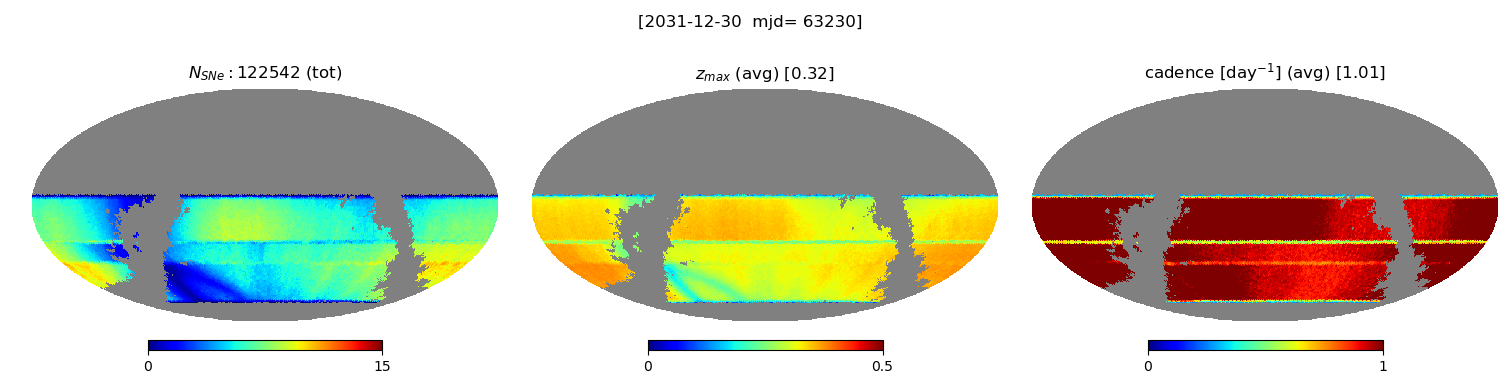
\includegraphics[width=\linewidth]{wfd_maps/altsched_rolling_good_weather_64_maps.png}
    \caption{{\bf AltSched rolling} cadence: {\em Left:} total number
      of well sampled SNe~Ia per healpixel {\em center:} average
      maximum redshift at which the normal SN is no longer well
      sampled {\em right:} average cadence delivered by the survey.}
    \label{fig:altsched_rolling_good_weather}
  \end{center}
\end{figure}


\begin{figure}[h!]
  \begin{center}
    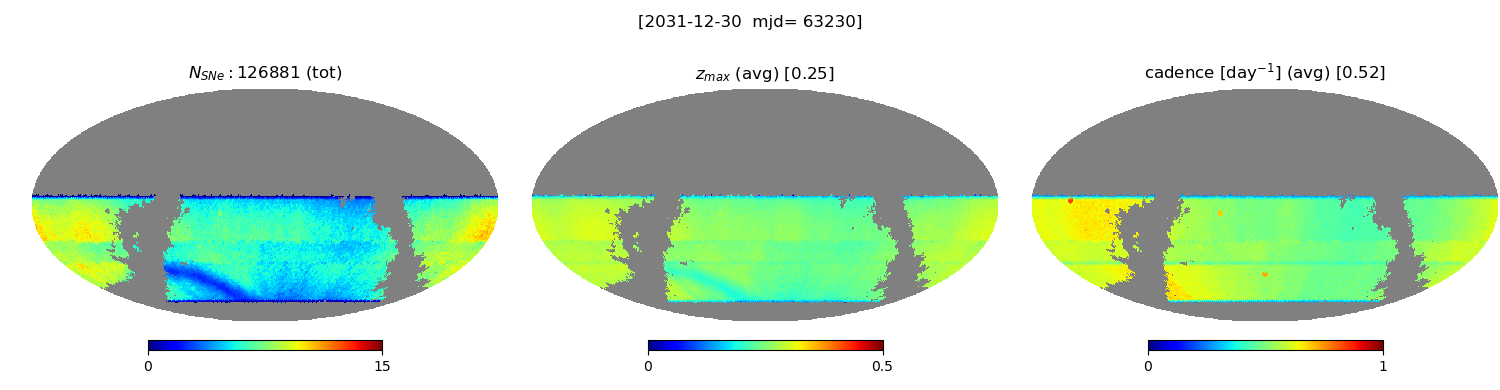
\includegraphics[width=\linewidth]{wfd_maps/altsched_good_weather_64_maps.png}
    \caption{{\bf AltSched} cadence: {\em Left:} total number of well
      sampled SNe~Ia per healpixel {\em center:} average maximum
      redshift at which the normal SN is no longer well sampled {\em
        right:} average cadence delivered by the survey.}
    \label{fig:altsched_good_weather}
  \end{center}
\end{figure}

\begin{figure}[h!]
  \begin{center}
    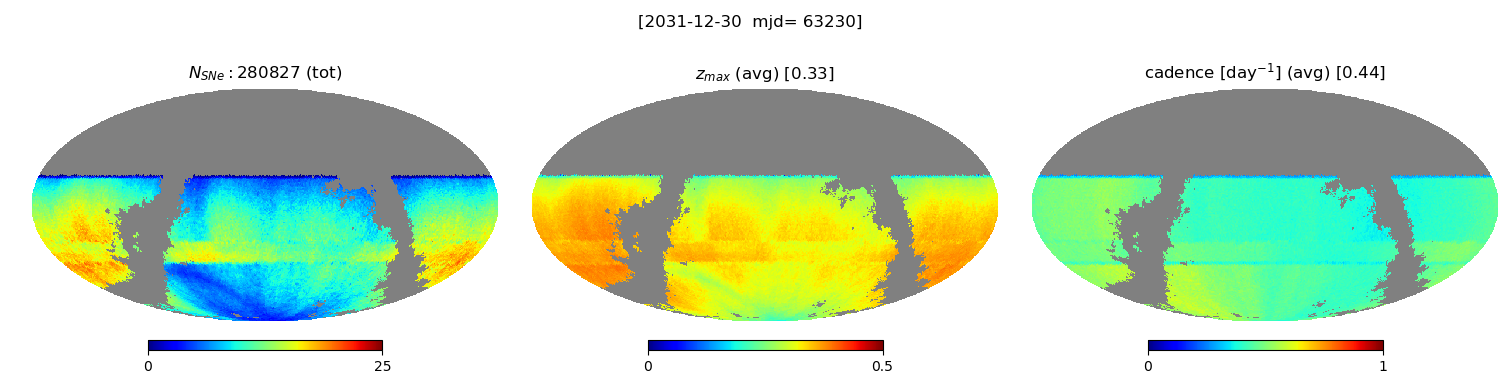
\includegraphics[width=\linewidth]{wfd_maps/altsched_18__90_40_64_maps.png}
    \caption{{\bf AltSched Wide} cadence: {\em Left:} total number of well
      sampled SNe~Ia per healpixel {\em center:} average maximum
      redshift at which the normal SN is no longer well sampled {\em
        right:} average cadence delivered by the survey.}
  \end{center}
  \label{fig:altsched_wide}
\end{figure}

\begin{figure}[h!]
  \begin{center}
    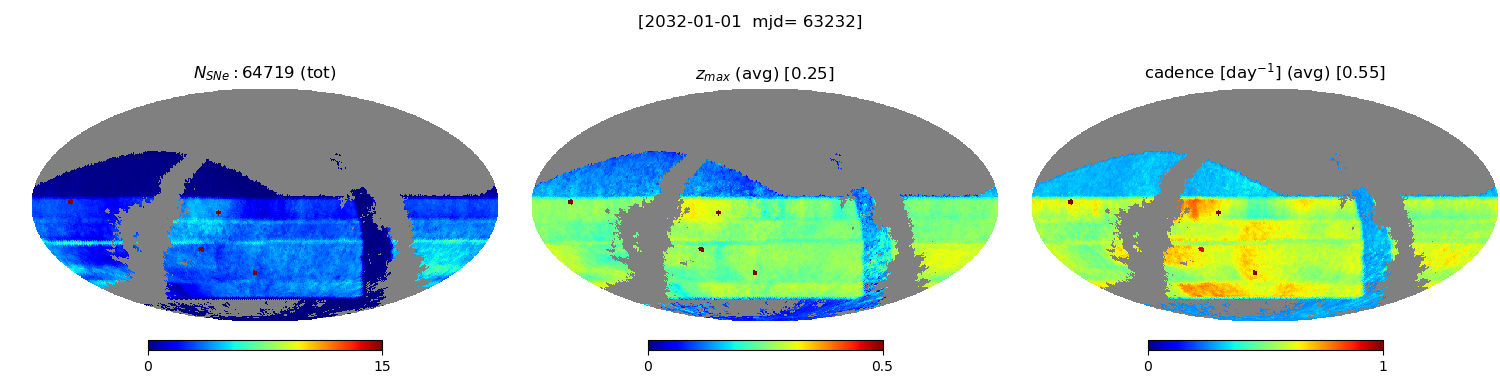
\includegraphics[width=\linewidth]{wfd_maps/tms_roll_10yrs_64_maps.png}
    \caption{{\bf SLAIR tms roll} cadence: {\em Left:} total number of well
      sampled SNe~Ia per healpixel {\em center:} average maximum
      redshift at which the normal SN is no longer well sampled {\em
        right:} average cadence delivered by the survey.}
    \label{fig:tms_roll}
  \end{center}
\end{figure}

\begin{figure}[h!]
  \begin{center}
    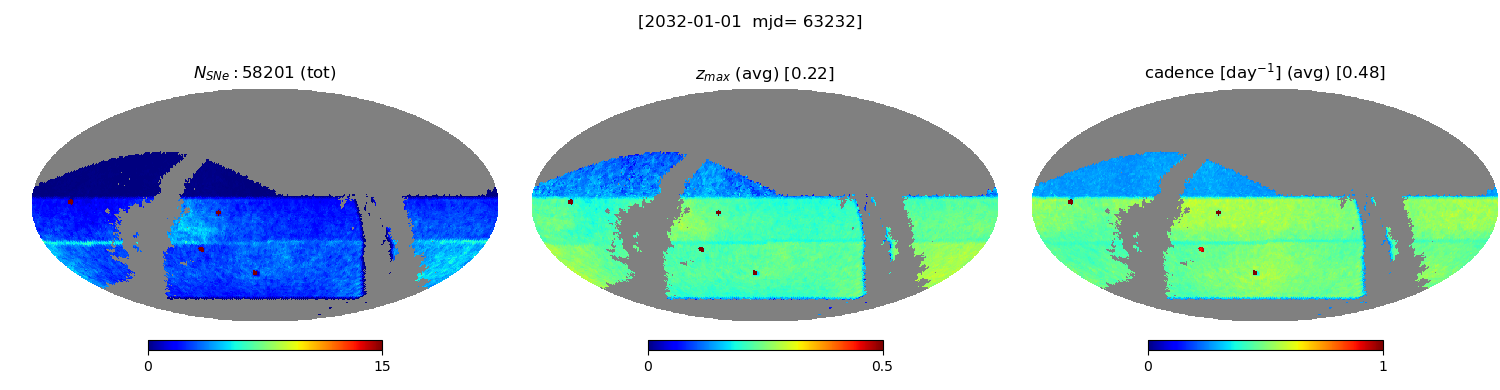
\includegraphics[width=\linewidth]{wfd_maps/rolling_mix_75_10yrs_64_maps.png}
    \caption{{\bf SLAIR: rolling mix 75} cadence: {\em Left:} total number of well
      sampled SNe~Ia per healpixel {\em center:} average maximum
      redshift at which the normal SN is no longer well sampled {\em
        right:} average cadence delivered by the survey.}
    \label{fig:rolling_mix_75}
  \end{center}
\end{figure}


\begin{figure}[h!]
  \begin{center}
    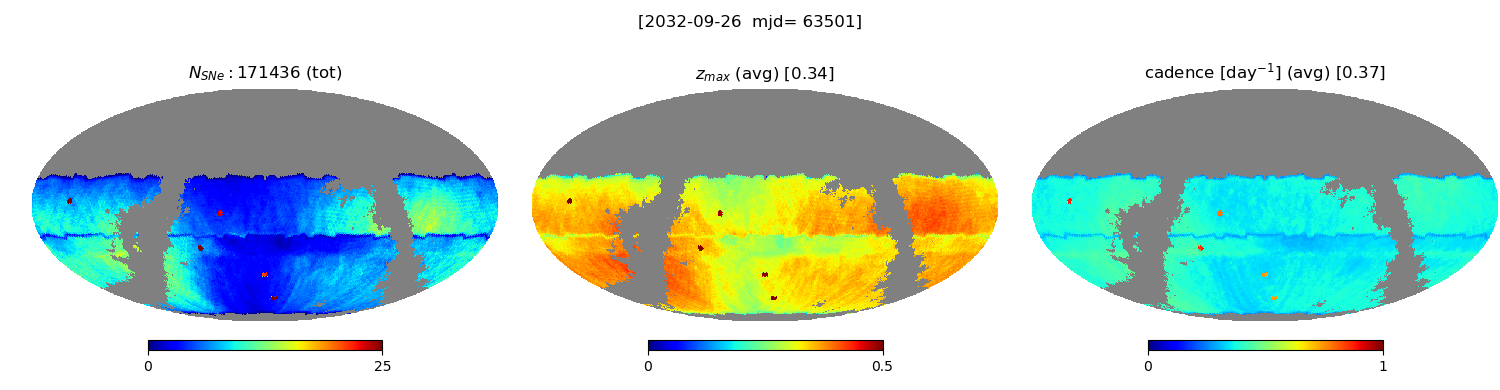
\includegraphics[width=\linewidth]{wfd_maps/mothra_2049_64_maps.png}
    \caption{{\bf Mothra 2049} cadence: {\em Left:} total number of well
      sampled SNe~Ia per healpixel {\em center:} average maximum
      redshift at which the normal SN is no longer well sampled {\em
        right:} average cadence delivered by the survey.}
    \label{fig:mothra_2049}
  \end{center}
\end{figure}

\begin{figure}[h!]
  \begin{center}
    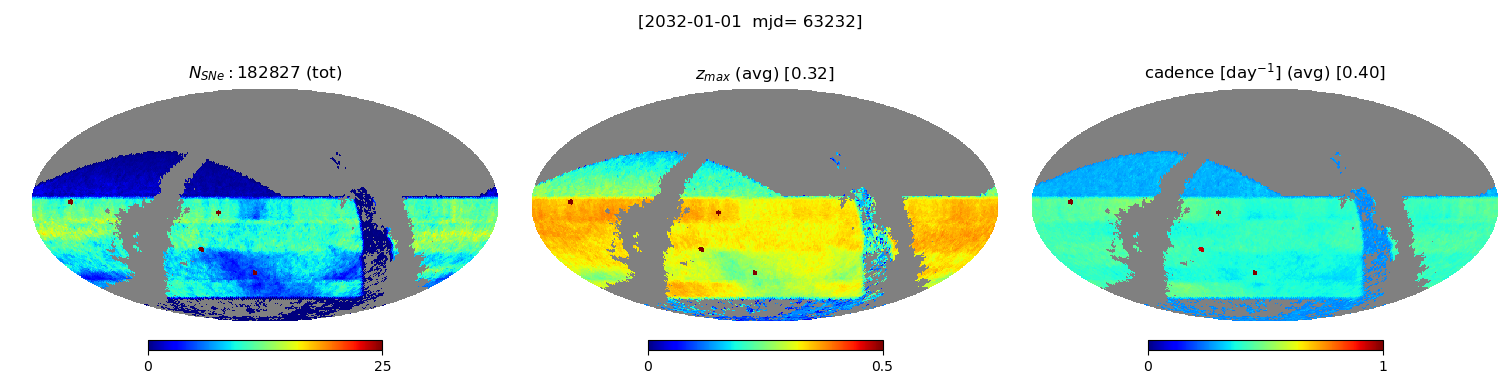
\includegraphics[width=\linewidth]{wfd_maps/tms_drive_10yrs_64_maps.png}
    \caption{{\bf SLAIR tms drive} cadence: {\em Left:} total number of well
      sampled SNe~Ia per healpixel {\em center:} average maximum
      redshift at which the normal SN is no longer well sampled {\em
        right:} average cadence delivered by the survey.}
    \label{fig:tms_drive}
  \end{center}
\end{figure}

\begin{figure}[h!]
  \begin{center}
    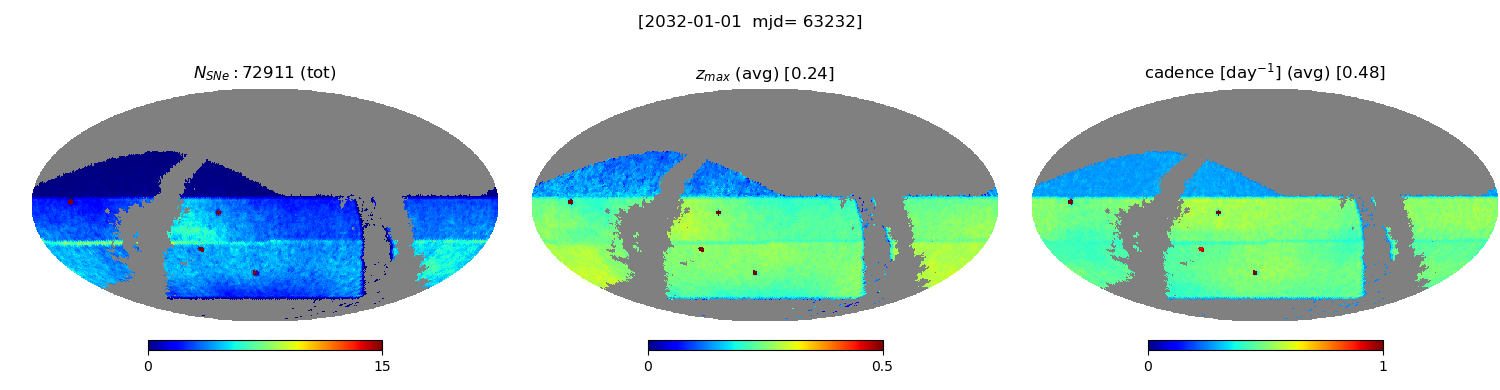
\includegraphics[width=\linewidth]{wfd_maps/rolling_mix_10yrs_64_maps.png}
    \caption{{\bf SLAIR: rolling mix} cadence: {\em Left:} total number of well
      sampled SNe~Ia per healpixel {\em center:} average maximum
      redshift at which the normal SN is no longer well sampled {\em
        right:} average cadence delivered by the survey.}
    \label{fig:rolling_mix}
  \end{center}
\end{figure}

\begin{figure}[h!]
  \begin{center}
    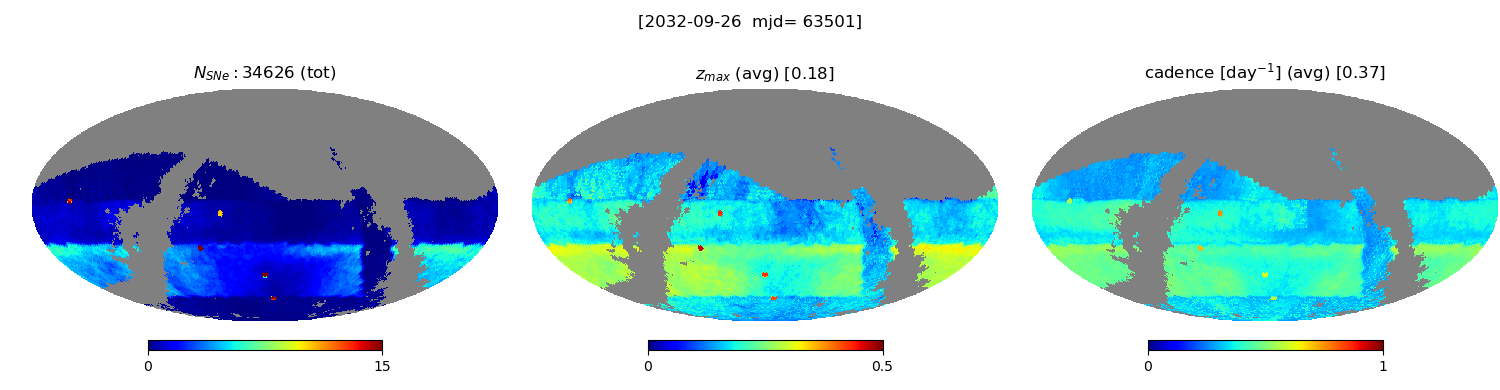
\includegraphics[width=\linewidth]{wfd_maps/mothra_2045_64_maps.png}
    \caption{{\bf Mothra 2045} cadence: {\em Left:} total number of well
      sampled SNe~Ia per healpixel {\em center:} average maximum
      redshift at which the normal SN is no longer well sampled {\em
        right:} average cadence delivered by the survey.}
    \label{fig:mothra_2045}
  \end{center}
\end{figure}

\begin{figure}[h!]
  \begin{center}
    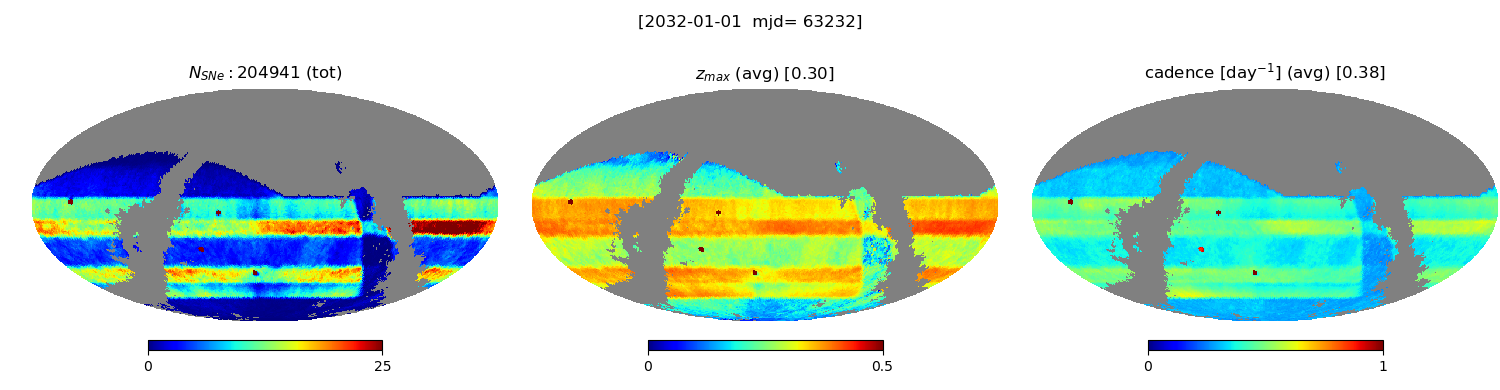
\includegraphics[width=\linewidth]{wfd_maps/tight_mask_10yrs_64_maps.png}
    \caption{{\bf SLAIR tight mask} cadence: {\em Left:} total number of well
      sampled SNe~Ia per healpixel {\em center:} average maximum
      redshift at which the normal SN is no longer well sampled {\em
        right:} average cadence delivered by the survey.}
    \label{fig:tight_mask}
  \end{center}
\end{figure}

\begin{figure}[h!]
  \begin{center}
    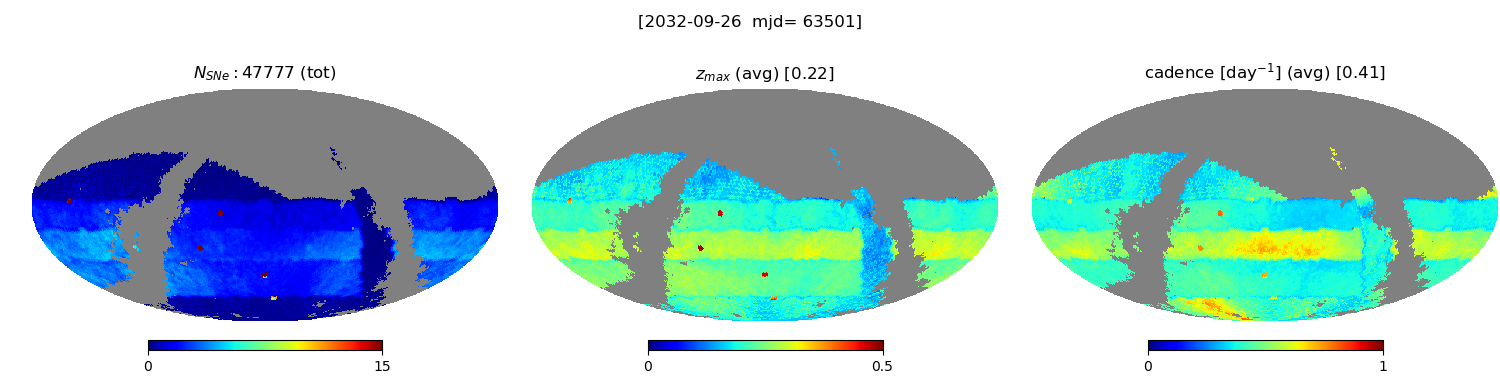
\includegraphics[width=\linewidth]{wfd_maps/kraken_2036_64_maps.png}
    \caption{{\bf Kraken 2036} cadence: {\em Left:} total number of well
      sampled SNe~Ia per healpixel {\em center:} average maximum
      redshift at which the normal SN is no longer well sampled {\em
        right:} average cadence delivered by the survey.}
    \label{fig:kraken_2036}
  \end{center}
\end{figure}

\begin{figure}[h!]
  \begin{center}
    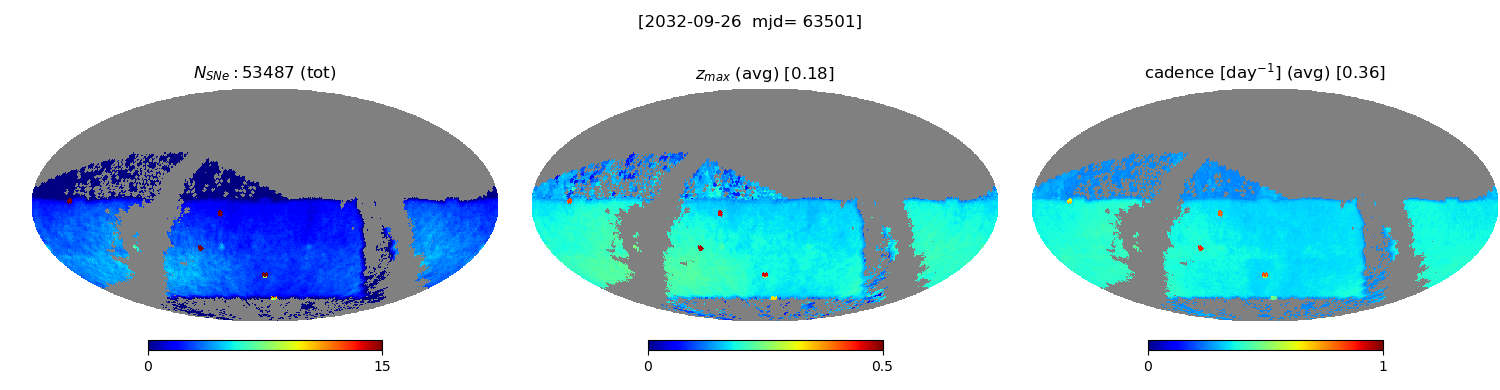
\includegraphics[width=\linewidth]{wfd_maps/pontus_2489_64_maps.png}
    \caption{{\bf Pontus 2489} cadence: {\em Left:} total number of well
      sampled SNe~Ia per healpixel {\em center:} average maximum
      redshift at which the normal SN is no longer well sampled {\em
        right:} average cadence delivered by the survey.}
    \label{fig:pontus_2489}
  \end{center}
\end{figure}

\begin{figure}[h!]
  \begin{center}
    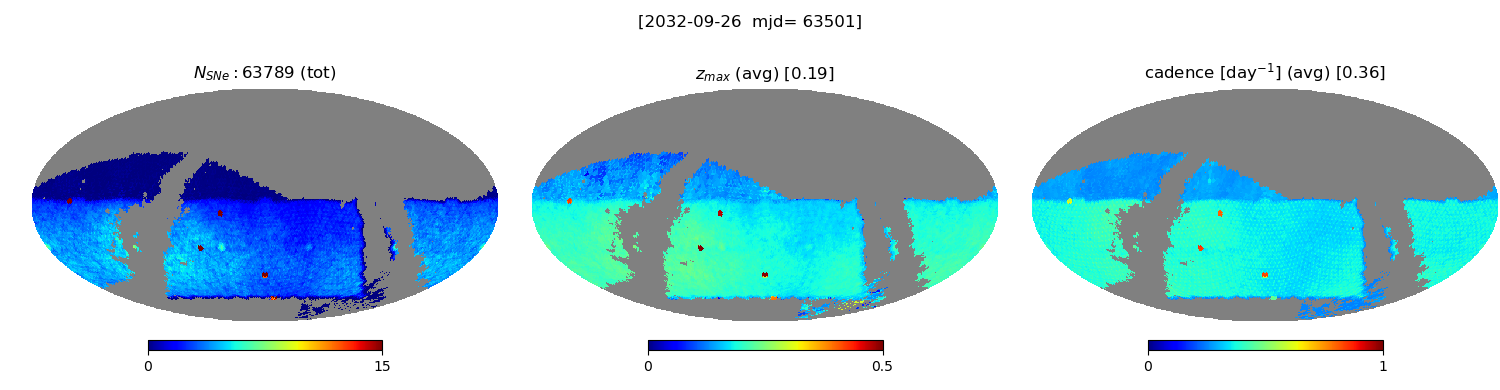
\includegraphics[width=\linewidth]{wfd_maps/colossus_2667_64_maps.png}
    \caption{{\bf Colossus 2667} cadence: {\em Left:} total number of well
      sampled SNe~Ia per healpixel {\em center:} average maximum
      redshift at which the normal SN is no longer well sampled {\em
        right:} average cadence delivered by the survey.}
  \end{center}
  \label{fig:colossus_2667}
\end{figure}

\begin{figure}[h!]
  \begin{center}
    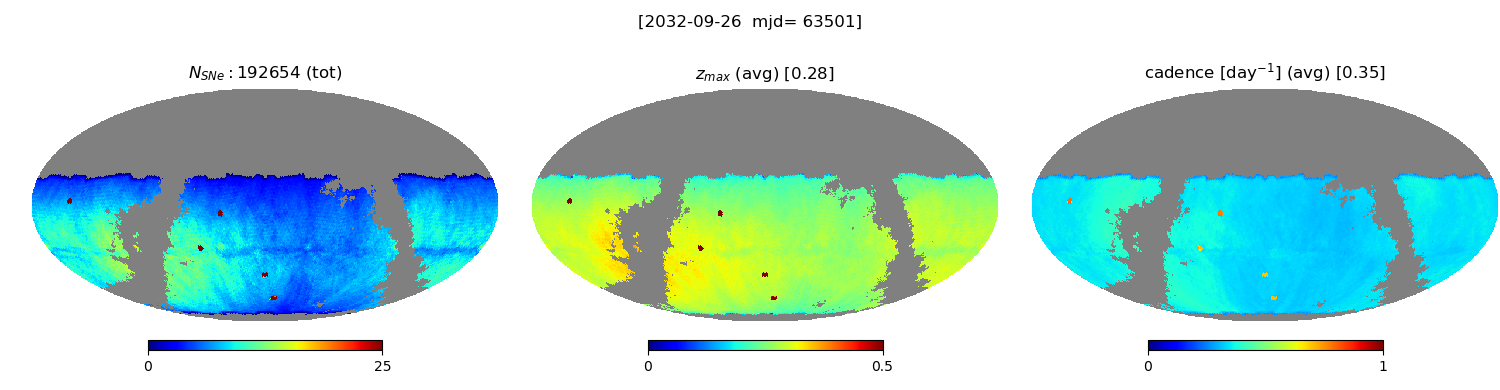
\includegraphics[width=\linewidth]{wfd_maps/kraken_2044_64_maps.png}
    \caption{{\bf Kraken 2044} cadence: {\em Left:} total number of well
      sampled SNe~Ia per healpixel {\em center:} average maximum
      redshift at which the normal SN is no longer well sampled {\em
        right:} average cadence delivered by the survey.}
    \label{fig:kraken_2044}
  \end{center}
\end{figure}

\begin{figure}[h!]
  \begin{center}
    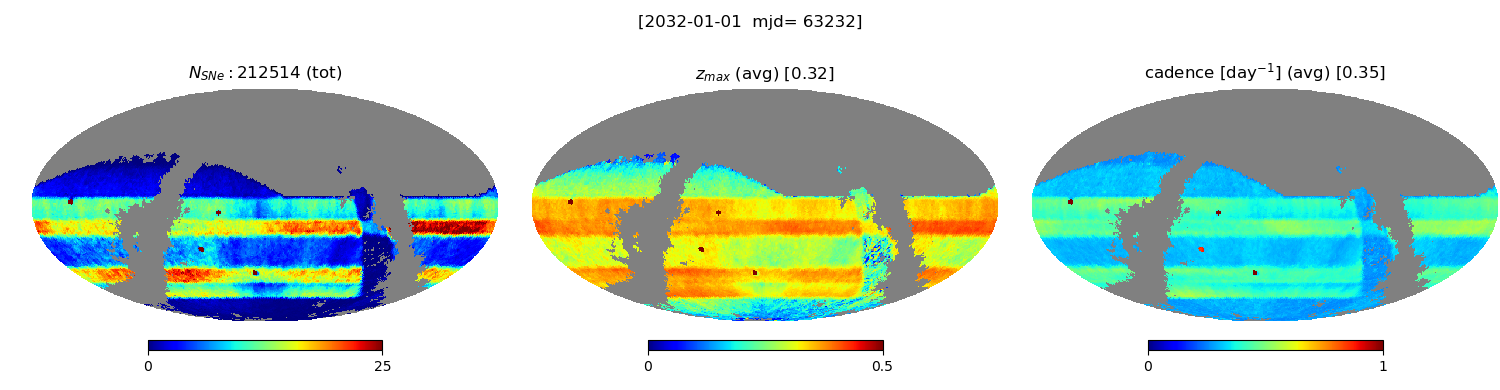
\includegraphics[width=\linewidth]{wfd_maps/tight_mask_simple_10yrs_64_maps.png}
    \caption{{\bf SLAIR tight mask simple} cadence: {\em Left:} total number of well
      sampled SNe~Ia per healpixel {\em center:} average maximum
      redshift at which the normal SN is no longer well sampled {\em
        right:} average cadence delivered by the survey.}
    \label{fig:tight_mask_simple}
  \end{center}
\end{figure}

\begin{figure}[h!]
  \begin{center}
    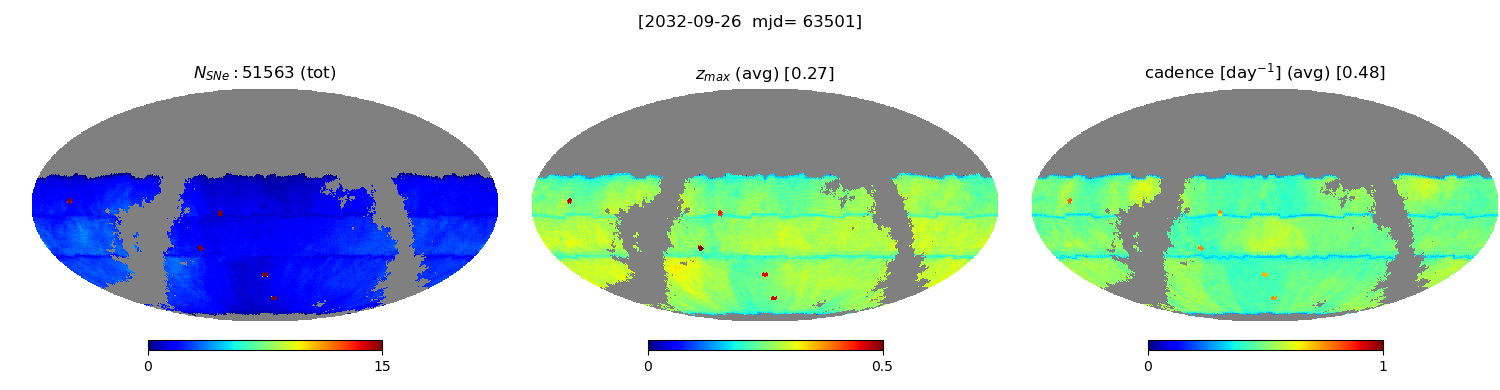
\includegraphics[width=\linewidth]{wfd_maps/nexus_2097_64_maps.png}
    \caption{{\bf Nexus 2097} cadence: {\em Left:} total number of well
      sampled SNe~Ia per healpixel {\em center:} average maximum
      redshift at which the normal SN is no longer well sampled {\em
        right:} average cadence delivered by the survey.}
    \label{fig:nexus_2097}
  \end{center}
\end{figure}

\begin{figure}[h!]
  \begin{center}
    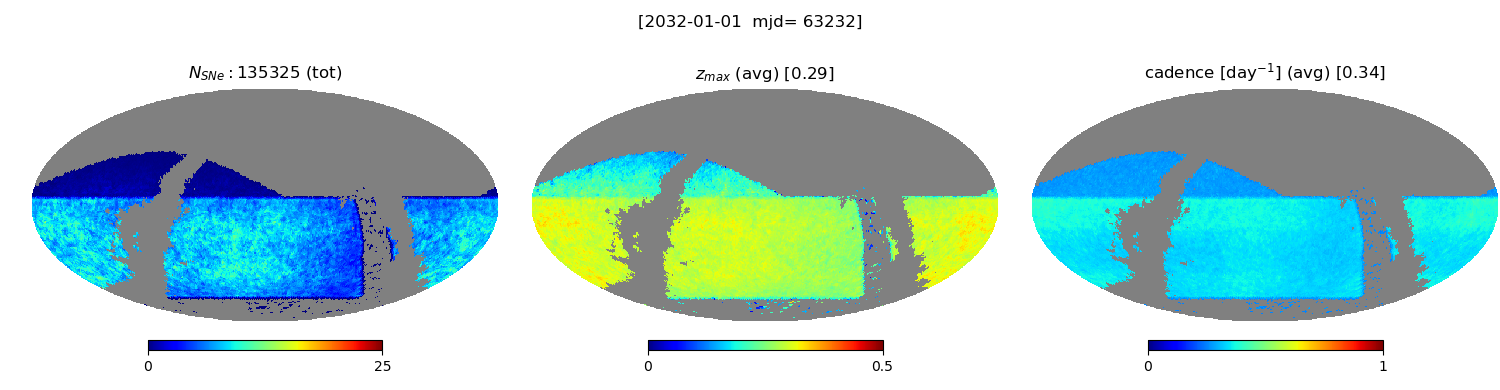
\includegraphics[width=\linewidth]{wfd_maps/cadence_mix_10yrs_64_maps.png}
    \caption{{\bf SLAIR: mix} cadence: {\em Left:} total number of well
      sampled SNe~Ia per healpixel {\em center:} average maximum
      redshift at which the normal SN is no longer well sampled {\em
        right:} average cadence delivered by the survey.}
    \label{fig:cadence_mix}
  \end{center}
\end{figure}

\begin{figure}[h!]
  \begin{center}
    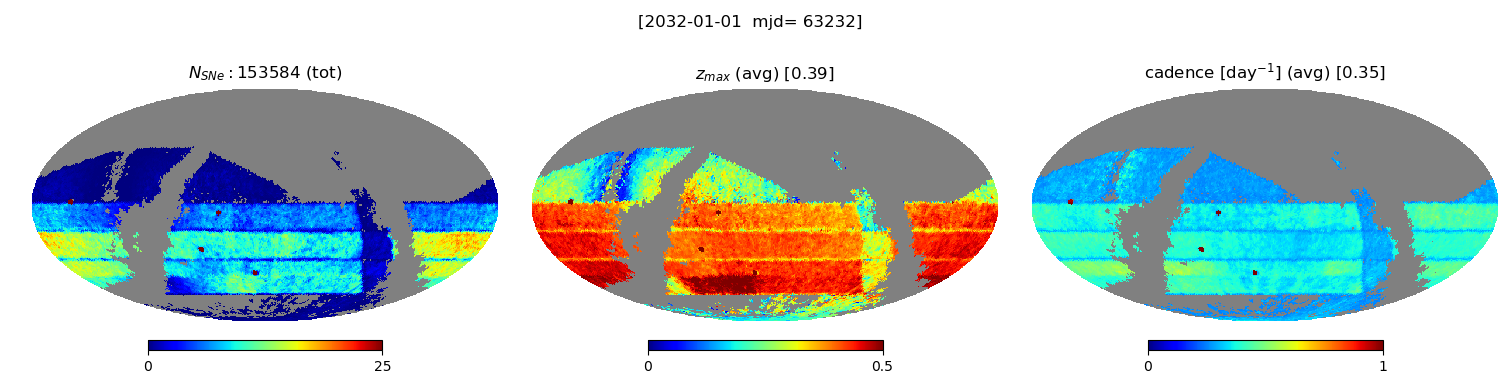
\includegraphics[width=\linewidth]{wfd_maps/feature_rolling_twoThird_10yrs_64_maps.png}
    \caption{{\bf Feature rolling 2/3} cadence: {\em Left:} total number of well
      sampled SNe~Ia per healpixel {\em center:} average maximum
      redshift at which the normal SN is no longer well sampled {\em
        right:} average cadence delivered by the survey.}
    \label{fig:feature_rolling_two_third}
  \end{center}
\end{figure}

\begin{figure}[h!]
  \begin{center}
    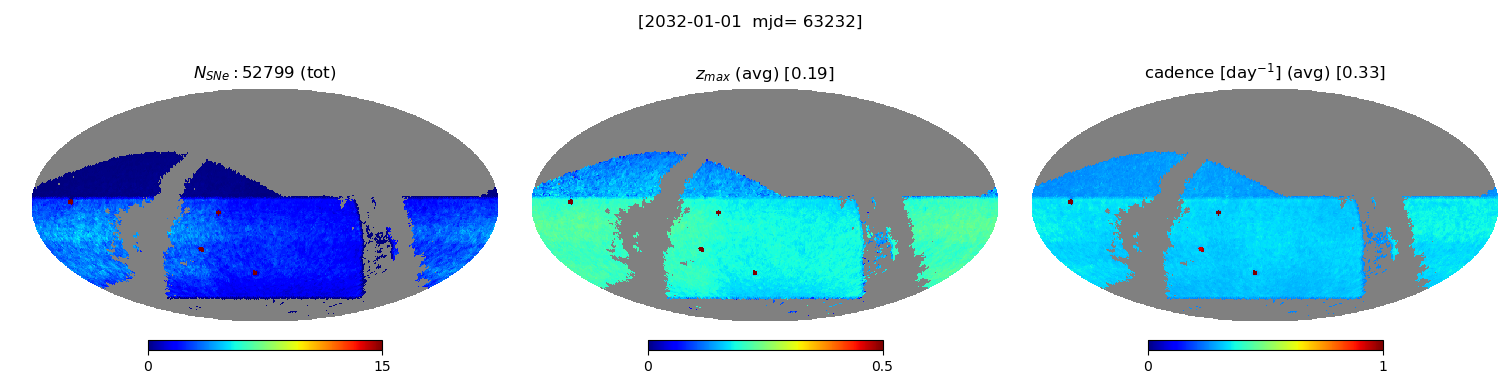
\includegraphics[width=\linewidth]{wfd_maps/blobs_mix_zmask10yrs_64_maps.png}
    \caption{{\bf SLAIR: blobs mix zmask} cadence: {\em Left:} total number of well
      sampled SNe~Ia per healpixel {\em center:} average maximum
      redshift at which the normal SN is no longer well sampled {\em
        right:} average cadence delivered by the survey.}
    \label{fig:blobs_mix_zmask}
  \end{center}
\end{figure}

\begin{figure}[h!]
  \begin{center}
    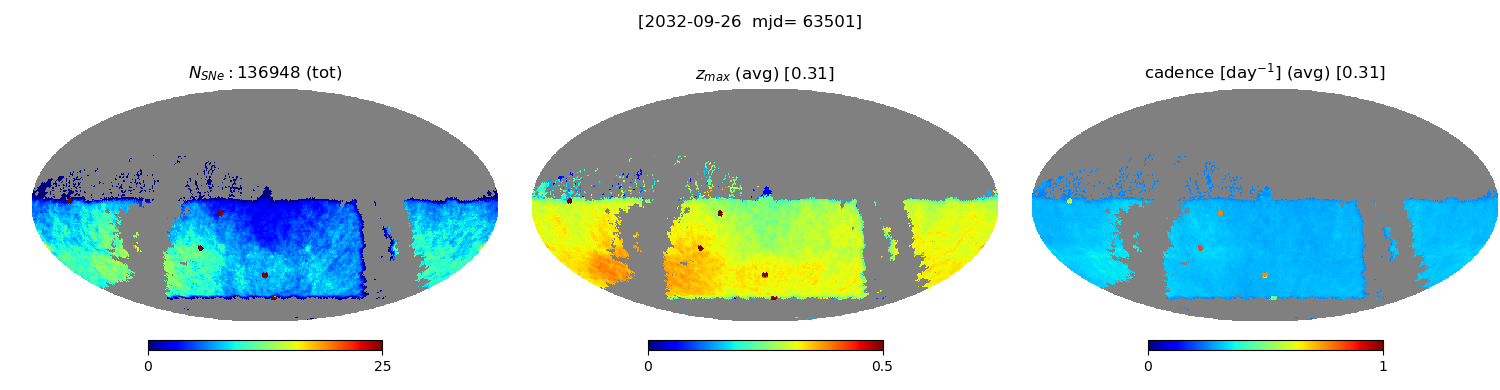
\includegraphics[width=\linewidth]{wfd_maps/kraken_2026_64_maps.png}
    \caption{{\bf Kraken 2026} cadence: {\em Left:} total number of well
      sampled SNe~Ia per healpixel {\em center:} average maximum
      redshift at which the normal SN is no longer well sampled {\em
        right:} average cadence delivered by the survey.}
  \end{center}
  \label{fig:kraken_2026}
\end{figure}

\begin{figure}[h!]
  \begin{center}
    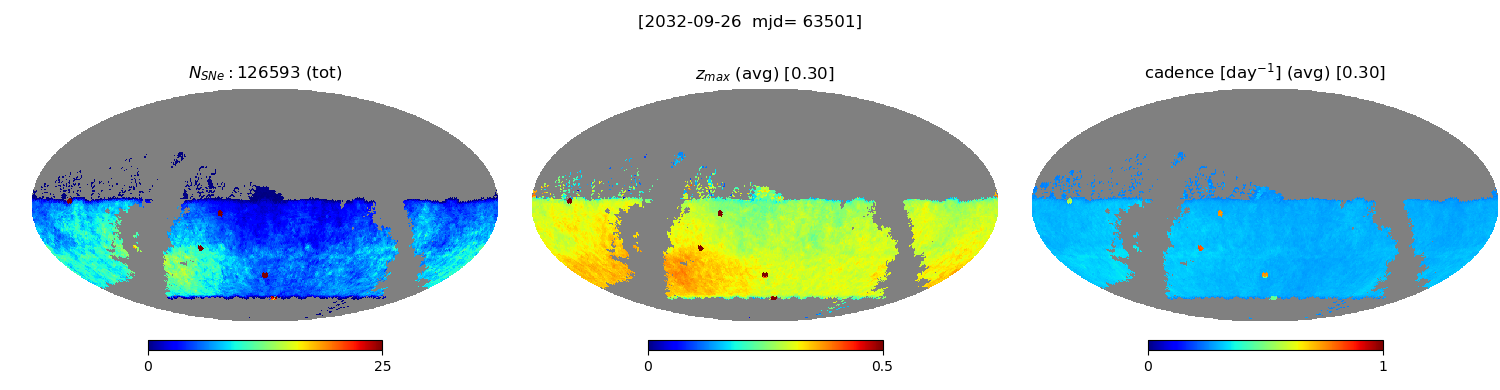
\includegraphics[width=\linewidth]{wfd_maps/colossus_2664_64_maps.png}
    \caption{{\bf Colossus 2664} cadence: {\em Left:} total number of well
      sampled SNe~Ia per healpixel {\em center:} average maximum
      redshift at which the normal SN is no longer well sampled {\em
        right:} average cadence delivered by the survey.}
    \label{fig:colossus_2664}
  \end{center}
\end{figure}

\begin{figure}[h!]
  \begin{center}
    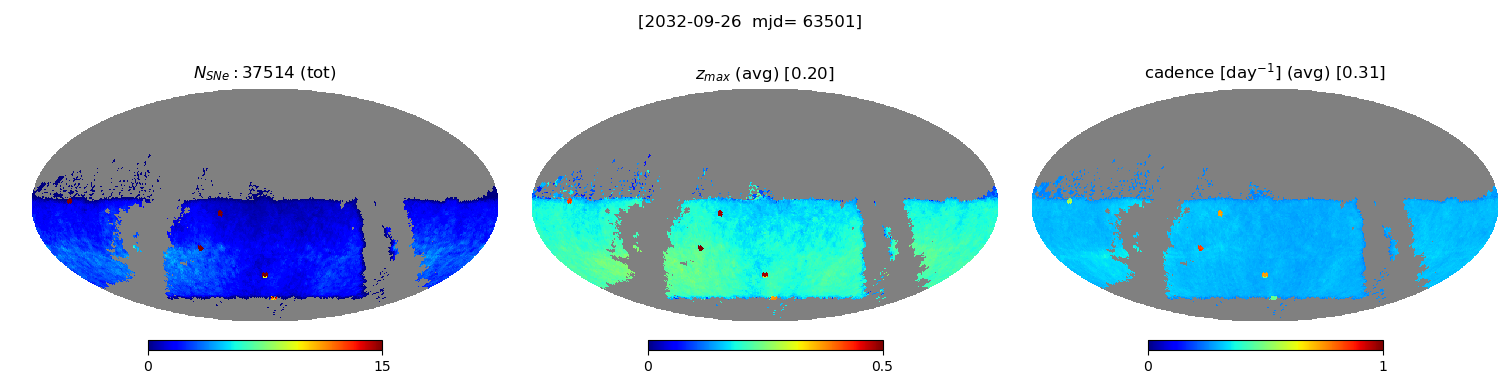
\includegraphics[width=\linewidth]{wfd_maps/baseline2018a_64_maps.png}
    \caption{{\bf Baseline 2018a} cadence: {\em Left:} total number of well
      sampled SNe~Ia per healpixel {\em center:} average maximum
      redshift at which the normal SN is no longer well sampled {\em
        right:} average cadence delivered by the survey.}
  \end{center}
  \label{fig:baseline2018}
\end{figure}

\begin{figure}[h!]
  \begin{center}
    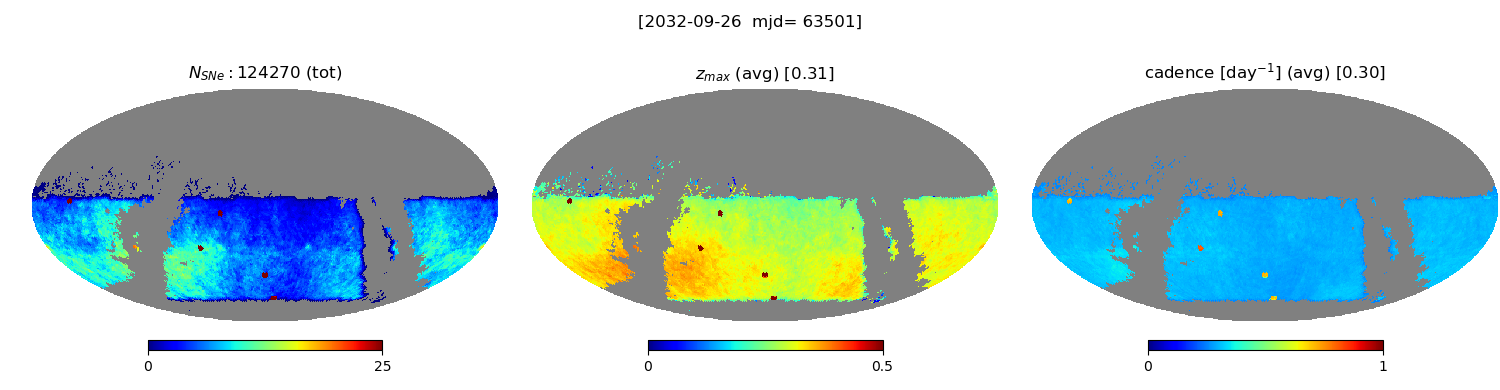
\includegraphics[width=\linewidth]{wfd_maps/colossus_2665_64_maps.png}
    \caption{{\bf Colossus 2665} cadence: {\em Left:} total number of well
      sampled SNe~Ia per healpixel {\em center:} average maximum
      redshift at which the normal SN is no longer well sampled {\em
        right:} average cadence delivered by the survey.}
  \end{center}
  \label{fig:colossus_2665}
\end{figure}

\begin{figure}[h!]
  \begin{center}
    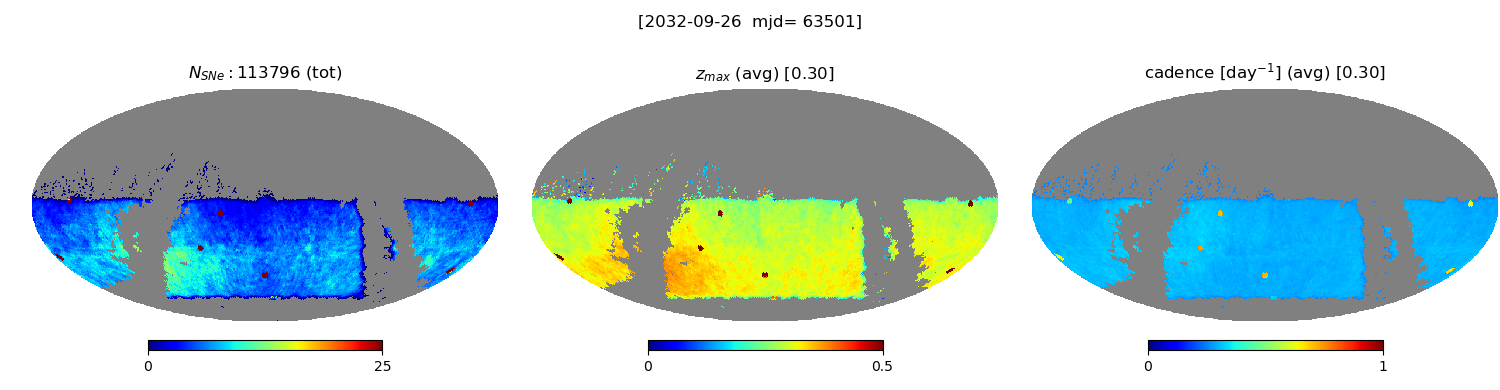
\includegraphics[width=\linewidth]{wfd_maps/kraken_2035_64_maps.png}
    \caption{{\bf Kraken 2035} cadence: {\em Left:} total number of well
      sampled SNe~Ia per healpixel {\em center:} average maximum
      redshift at which the normal SN is no longer well sampled {\em
        right:} average cadence delivered by the survey.}
  \end{center}
  \label{fig:kraken_2035}
\end{figure}

\begin{figure}[h!]
  \begin{center}
    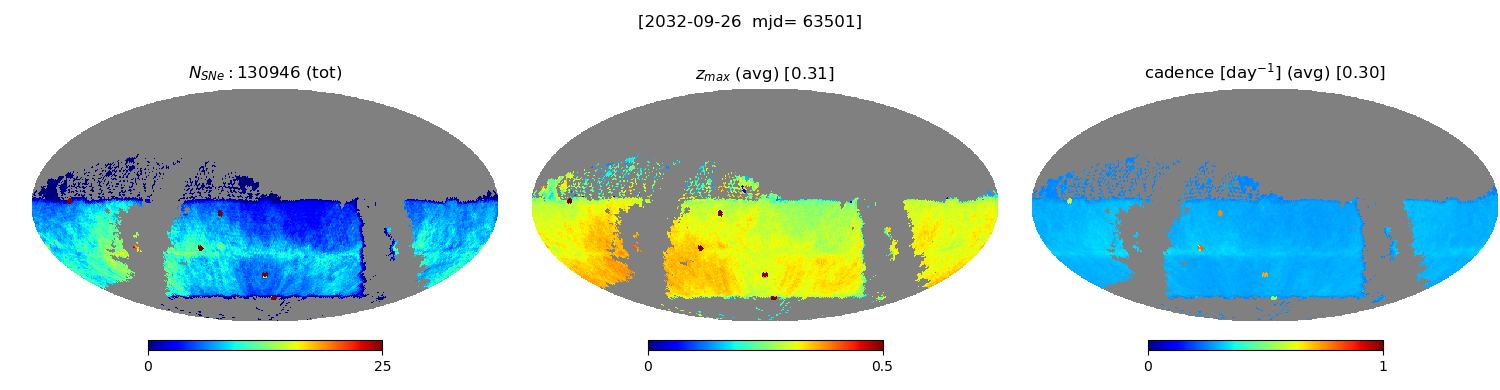
\includegraphics[width=\linewidth]{wfd_maps/kraken_2042_64_maps.png}
    \caption{{\bf Kraken 2042} cadence: {\em Left:} total number of well
      sampled SNe~Ia per healpixel {\em center:} average maximum
      redshift at which the normal SN is no longer well sampled {\em
        right:} average cadence delivered by the survey.}
    \label{fig:kraken_2042}
  \end{center}
\end{figure}

\begin{figure}[h!]
  \begin{center}
    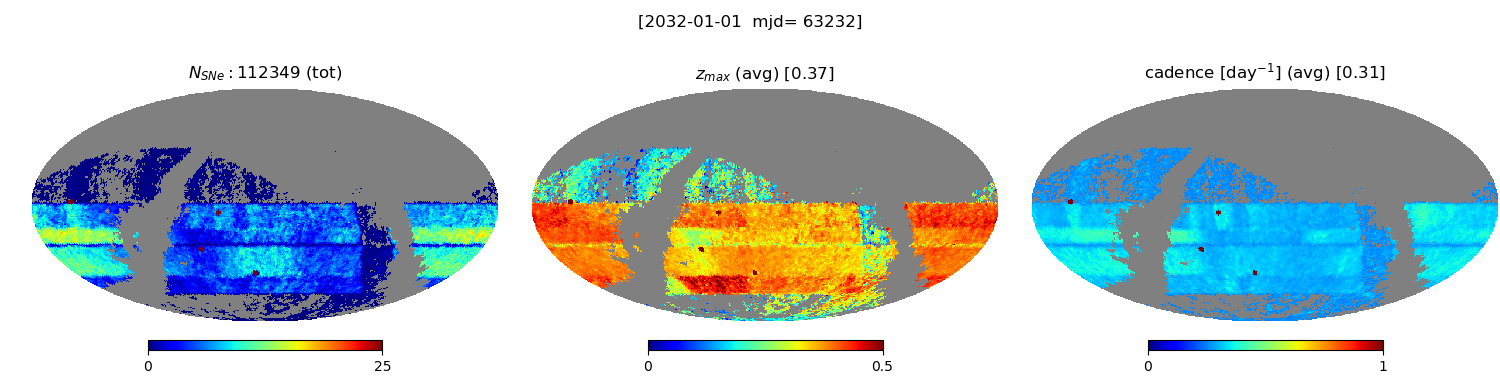
\includegraphics[width=\linewidth]{wfd_maps/feature_rolling_half_mask_10yrs_64_maps.png}
    \caption{{\bf Feature rolling 1/2} cadence: {\em Left:} total number of well
      sampled SNe~Ia per healpixel {\em center:} average maximum
      redshift at which the normal SN is no longer well sampled {\em
        right:} average cadence delivered by the survey.}
    \label{fig:feature_rolling_half_mask}
  \end{center}
\end{figure}


\begin{figure}[h!]
  \begin{center}
    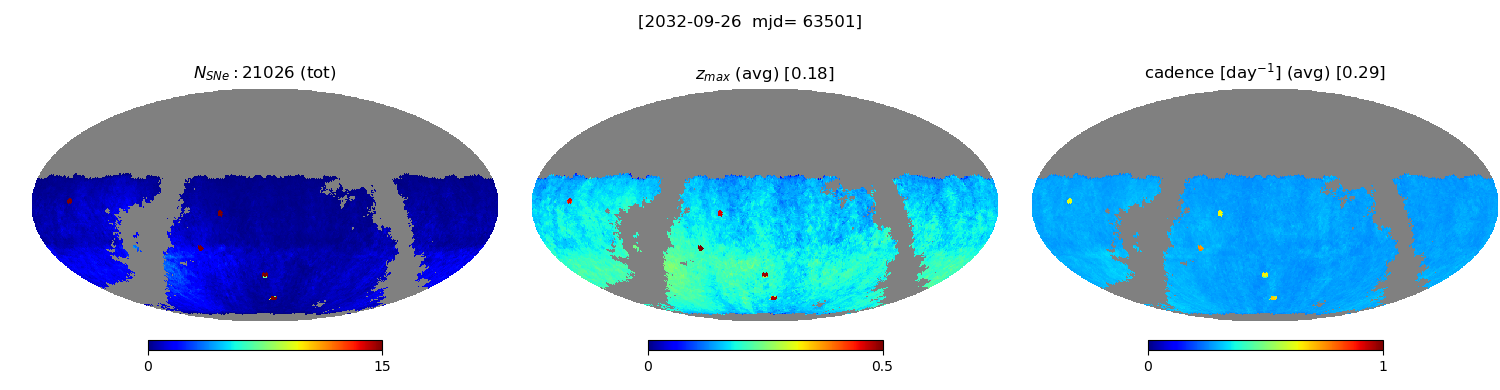
\includegraphics[width=\linewidth]{wfd_maps/pontus_2002_64_maps.png}
    \caption{{\bf Pontus 2002} cadence: {\em Left:} total number of well
      sampled SNe~Ia per healpixel {\em center:} average maximum
      redshift at which the normal SN is no longer well sampled {\em
        right:} average cadence delivered by the survey.}
    \label{fig:pontus_2002}
  \end{center}
\end{figure}

\begin{figure}[h!]
  \begin{center}
    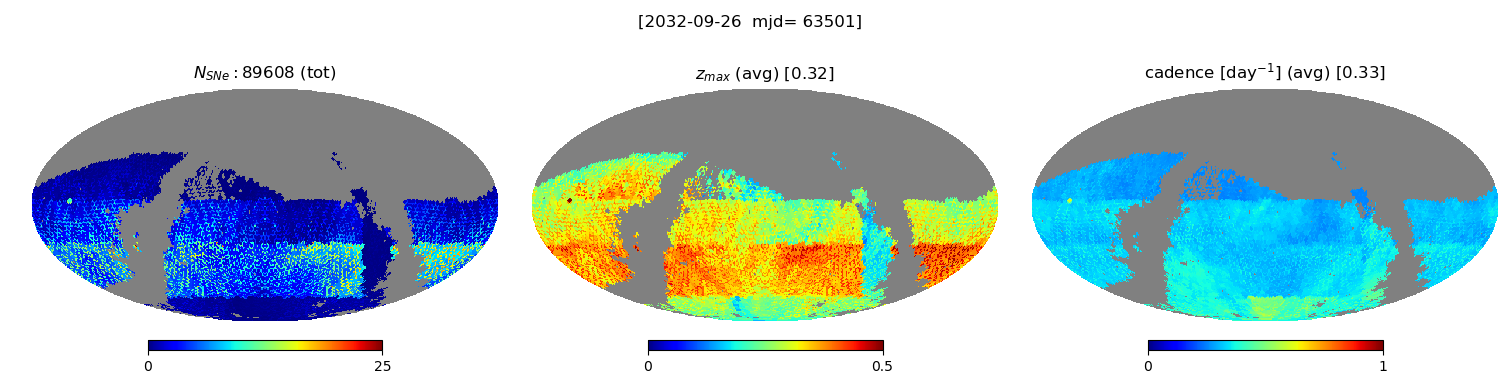
\includegraphics[width=\linewidth]{wfd_maps/pontus_2502_64_maps.png}
    \caption{{\bf Pontus 2502} cadence: {\em Left:} total number of well
      sampled SNe~Ia per healpixel {\em center:} average maximum
      redshift at which the normal SN is no longer well sampled {\em
        right:} average cadence delivered by the survey.}
    \label{fig:pontus_2502}
  \end{center}
\end{figure}

\begin{figure}[h!]
  \begin{center}
    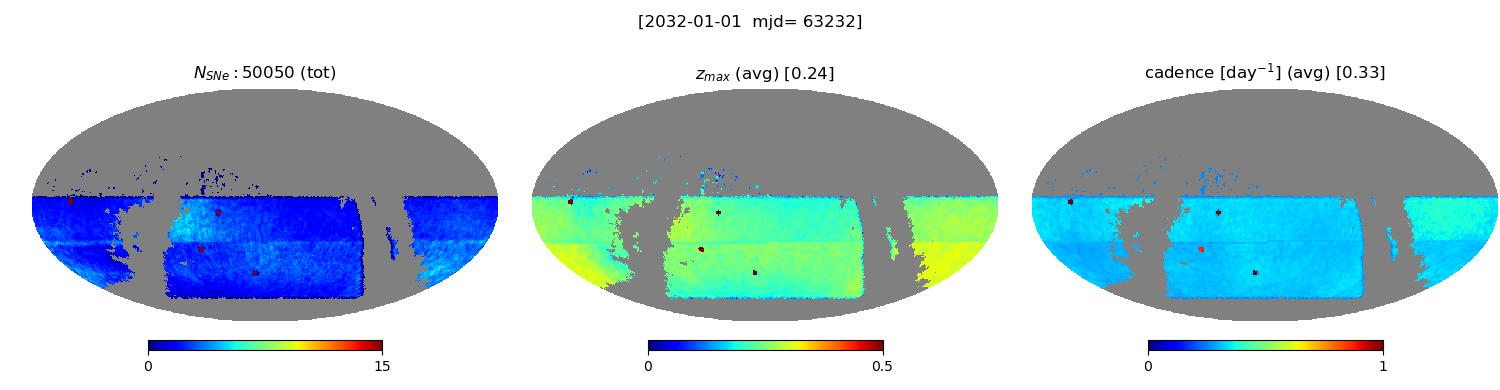
\includegraphics[width=\linewidth]{wfd_maps/rolling_10yrs_64_maps.png}
    \caption{{\bf SLAIR: rolling} cadence: {\em Left:} total number of well
      sampled SNe~Ia per healpixel {\em center:} average maximum
      redshift at which the normal SN is no longer well sampled {\em
        right:} average cadence delivered by the survey.}
    \label{fig:slair_rolling}
  \end{center}
\end{figure}

\begin{figure}[h!]
  \begin{center}
    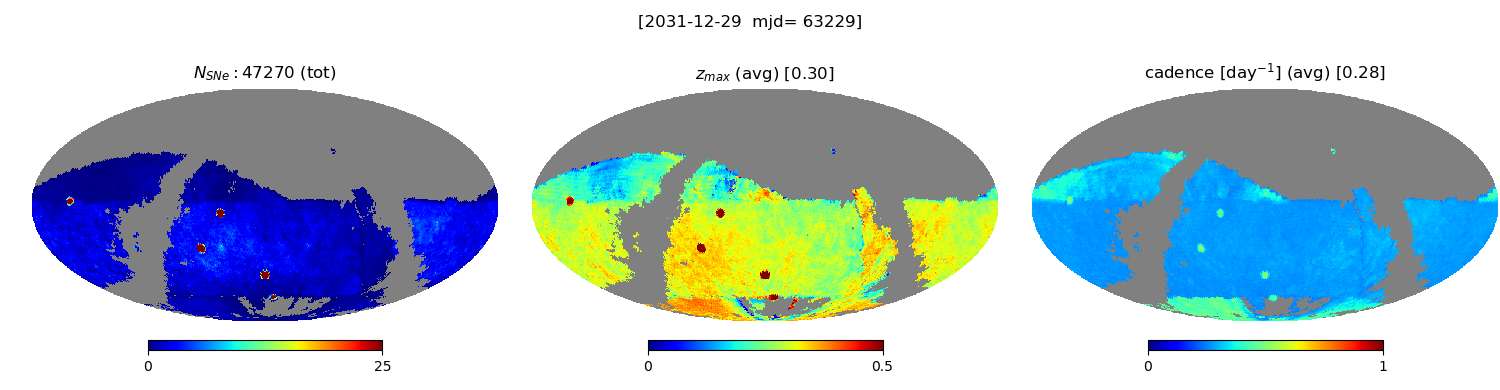
\includegraphics[width=\linewidth]{wfd_maps/minion_1016_64_maps.png}
    \caption{{\bf Minion 1016} cadence: {\em Left:} total number of well
      sampled SNe~Ia per healpixel {\em center:} average maximum
      redshift at which the normal SN is no longer well sampled {\em
        right:} average cadence delivered by the survey.}
    \label{fig:minion_1016}
  \end{center}
\end{figure}

\begin{figure}[h!]
  \begin{center}
    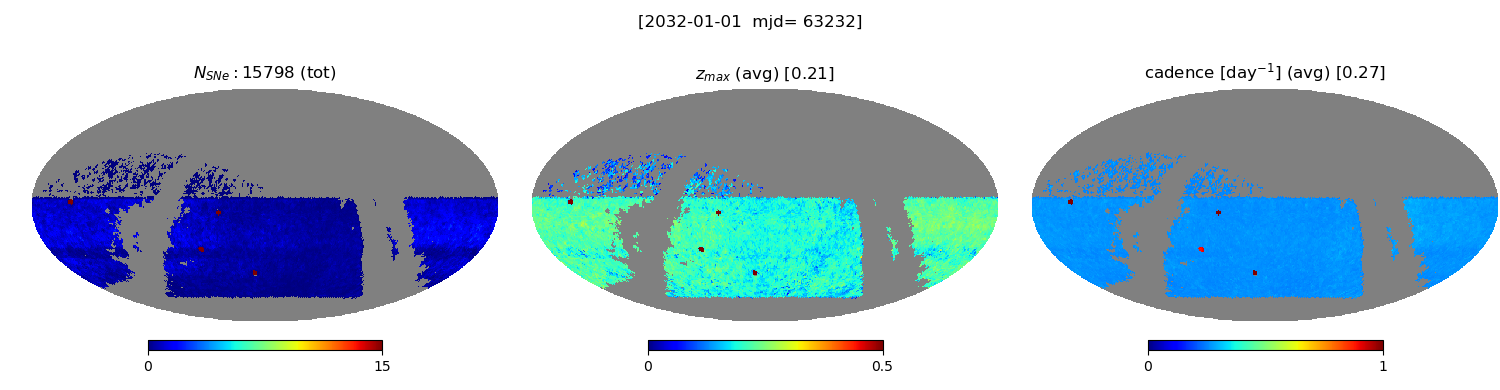
\includegraphics[width=\linewidth]{wfd_maps/blobs_same_10yrs_64_maps.png}
    \caption{{\bf SLAIR: blobs same} cadence: {\em Left:} total number of well
      sampled SNe~Ia per healpixel {\em center:} average maximum
      redshift at which the normal SN is no longer well sampled {\em
        right:} average cadence delivered by the survey.}
    \label{fig:blobs_same}
  \end{center}
\end{figure}

\begin{figure}[h!]
  \begin{center}
    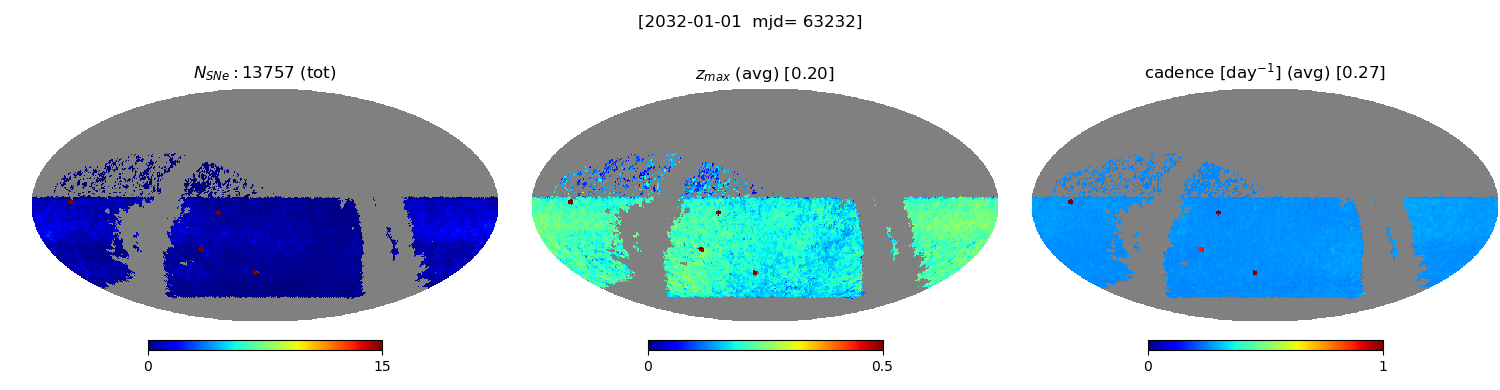
\includegraphics[width=\linewidth]{wfd_maps/blobs_same_zmask10yrs_64_maps.png}
    \caption{{\bf SLAIR: blobs same zmask} cadence: {\em Left:} total number of well
      sampled SNe~Ia per healpixel {\em center:} average maximum
      redshift at which the normal SN is no longer well sampled {\em
        right:} average cadence delivered by the survey.}
    \label{fig:blobs_same_zmask}
  \end{center}
\end{figure}

\begin{figure}[h!]
  \begin{center}
    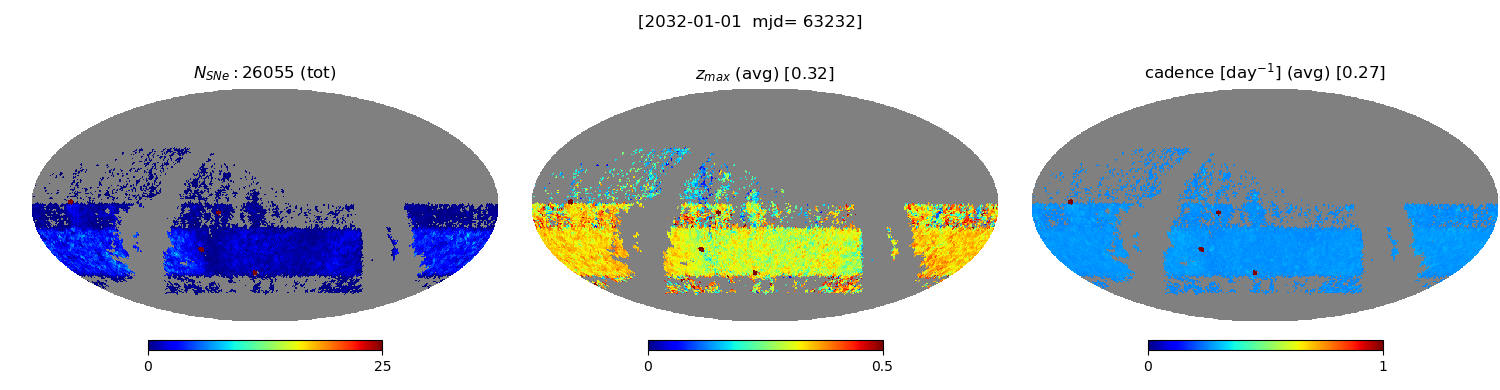
\includegraphics[width=\linewidth]{wfd_maps/feature_baseline_10yrs_64_maps.png}
    \caption{{\bf Feature baseline} cadence: {\em Left:} total number of well
      sampled SNe~Ia per healpixel {\em center:} average maximum
      redshift at which the normal SN is no longer well sampled {\em
        right:} average cadence delivered by the survey.}
    \label{fig:feature_baseline}
  \end{center}
\end{figure}






    
  \section{DDF plots}

  \input DD_plots_cadence.tex

\end{appendices}

\end{document}
